\chapter{海马体和外显记忆存储的神经基础} \label{chap:chap54}

外显记忆——有意识地回忆关于人、地点、物体和事件的信息——是人们通常认为的记忆。
有时称为陈述性记忆,它通过让我们随意回忆早餐吃了什么、在哪里吃以及和谁一起吃,将我们的精神生活联系在一起。
它使我们能够将今天所做的与昨天或前一周或前一个月所做的结合起来。


哺乳动物大脑中的两个结构对于编码和存储外显记忆尤为重要:前额皮质和海马体(第~\ref{chap:chap52}~章)。
前额叶皮层调解工作记忆,它只能在很短的时间内主动维持,然后很快就会被遗忘,例如只有在输入时才会记住的密码。
工作记忆中的信息可以作为长期记忆存储在大脑的其他地方,持续时间从几天到几周到几年,甚至贯穿一生。
虽然外显记忆的长期存储需要海马体,但大多数陈述性记忆的最终存储位置被认为是大脑皮层。


在本章中,我们将重点关注海马体的细胞、分子和网络机制,这些机制是外显记忆长期存储的基础。
由于海马体从称为内嗅皮层的大脑皮层区域接收其主要输入,该区域处理多种形式的感觉输入,因此我们还考虑了海马体如何转换来自内嗅皮层的信息。
特别是,我们研究了内嗅皮层和海马体中的神经活动如何通过编码动物在其环境中的位置表示来促进空间记忆。



\section{哺乳动物的外显记忆涉及海马体的突触可塑性}

与被认为由前额叶皮层中持续的神经活动维持的工作记忆不同(第 \ref{chap:chap52} 章),信息的长期存储被认为取决于特定神经元集合之间连接强度的长期变化( 神经组件)在海马体中编码特定的记忆元素。


记忆存储涉及大脑中持久的结构变化的想法,最早在 20 世纪初被德国生物学家理查德西蒙称为“印迹”,可以追溯到法国哲学家勒内笛卡尔。
为了找到记忆痕迹,美国心理学家卡尔·拉什利 (Karl Lashley) 研究了新皮质不同区域的病变对老鼠学习迷宫导航能力的影响。
由于迷宫中的表现似乎与病变的大小成正比,而不是与病变的精确位置成正比,因此拉什利得出结论,任何记忆痕迹都必须分布在整个大脑中。
尽管现在普遍认为外显记忆的存储分布在整个新皮质中,但也很明显,存储记忆的过程需要海马体,正如 Brenda Milner 对 H.M. 患者的开创性研究所证明的那样。
(第 \ref{chap:chap52} 章)以及随后对海马体有针对性损伤的动物进行的研究。
因此,了解大脑如何存储外显记忆取决于对皮质-海马体回路如何处理和存储信息的了解。


记忆存储的基本机制的性质过去是,现在仍然是心理学家和神经科学家之间许多猜测和争论的主题。
加拿大心理学家唐纳德·赫布 (Donald Hebb) 提出了一个有影响力的理论,他在 1949 年提出,当突触连接根据经验得到加强时,可能会产生记忆编码神经组件。 根据 Hebb 规则:“当细胞 A 的轴突。 . . 激发细胞 B 并反复或持续参与激发它,一个或两个细胞发生一些生长过程或代谢变化,从而提高 A 作为激发 B 的细胞之一的效率。” 
Hebb 规则的关键要素是要求突触前和突触后放电同时发生,因此该规则有时被改写为“一起放电的细胞,连接在一起”。
一个类似的赫布巧合原理被认为与发育后期突触连接的微调有关(第 \ref{chap:chap49} 章)。
Hebb 的想法后来由理论神经科学家 David Marr 根据对海马回路的考虑进行了完善。


海马体包含一个连接回路,可处理来自附近内嗅皮质表层的多模式感觉和空间信息。
该信息在到达海马体 CA1 区(海马体的主要输出区域)之前通过多个突触。
CA1 神经元在学习和记忆中的至关重要性可见于仅在该区域有病变的患者所表现出的深度记忆丧失,这一观察结果得到了许多动物研究的支持。
来自内嗅皮层的信息沿着两条兴奋通路到达 CA1 神经元,一条是直接的,一条是间接的。


在间接通路中,内嗅皮层 II 层神经元的轴突通过穿孔通路投射,以激发齿状回(海马体的一部分)的颗粒细胞。
接下来,颗粒细胞的轴突投射在苔藓纤维通路中,以激发海马 CA3 区域的锥体细胞。
最后,CA3 神经元的轴突通过 Schaffer 侧支通路投射,在 CA1 锥体细胞树突的更近端区域形成兴奋性突触(图 \ref{fig:54_1})。
(由于其三个连续的兴奋性突触连接,间接通路通常被称为三突触通路)。
最后,CA1 锥体细胞投射回内嗅皮层的深层并向前投射到下托,这是另一个连接海马体和广泛多样的大脑区域的内侧颞叶结构。


\begin{figure}[htbp]
	\centering
	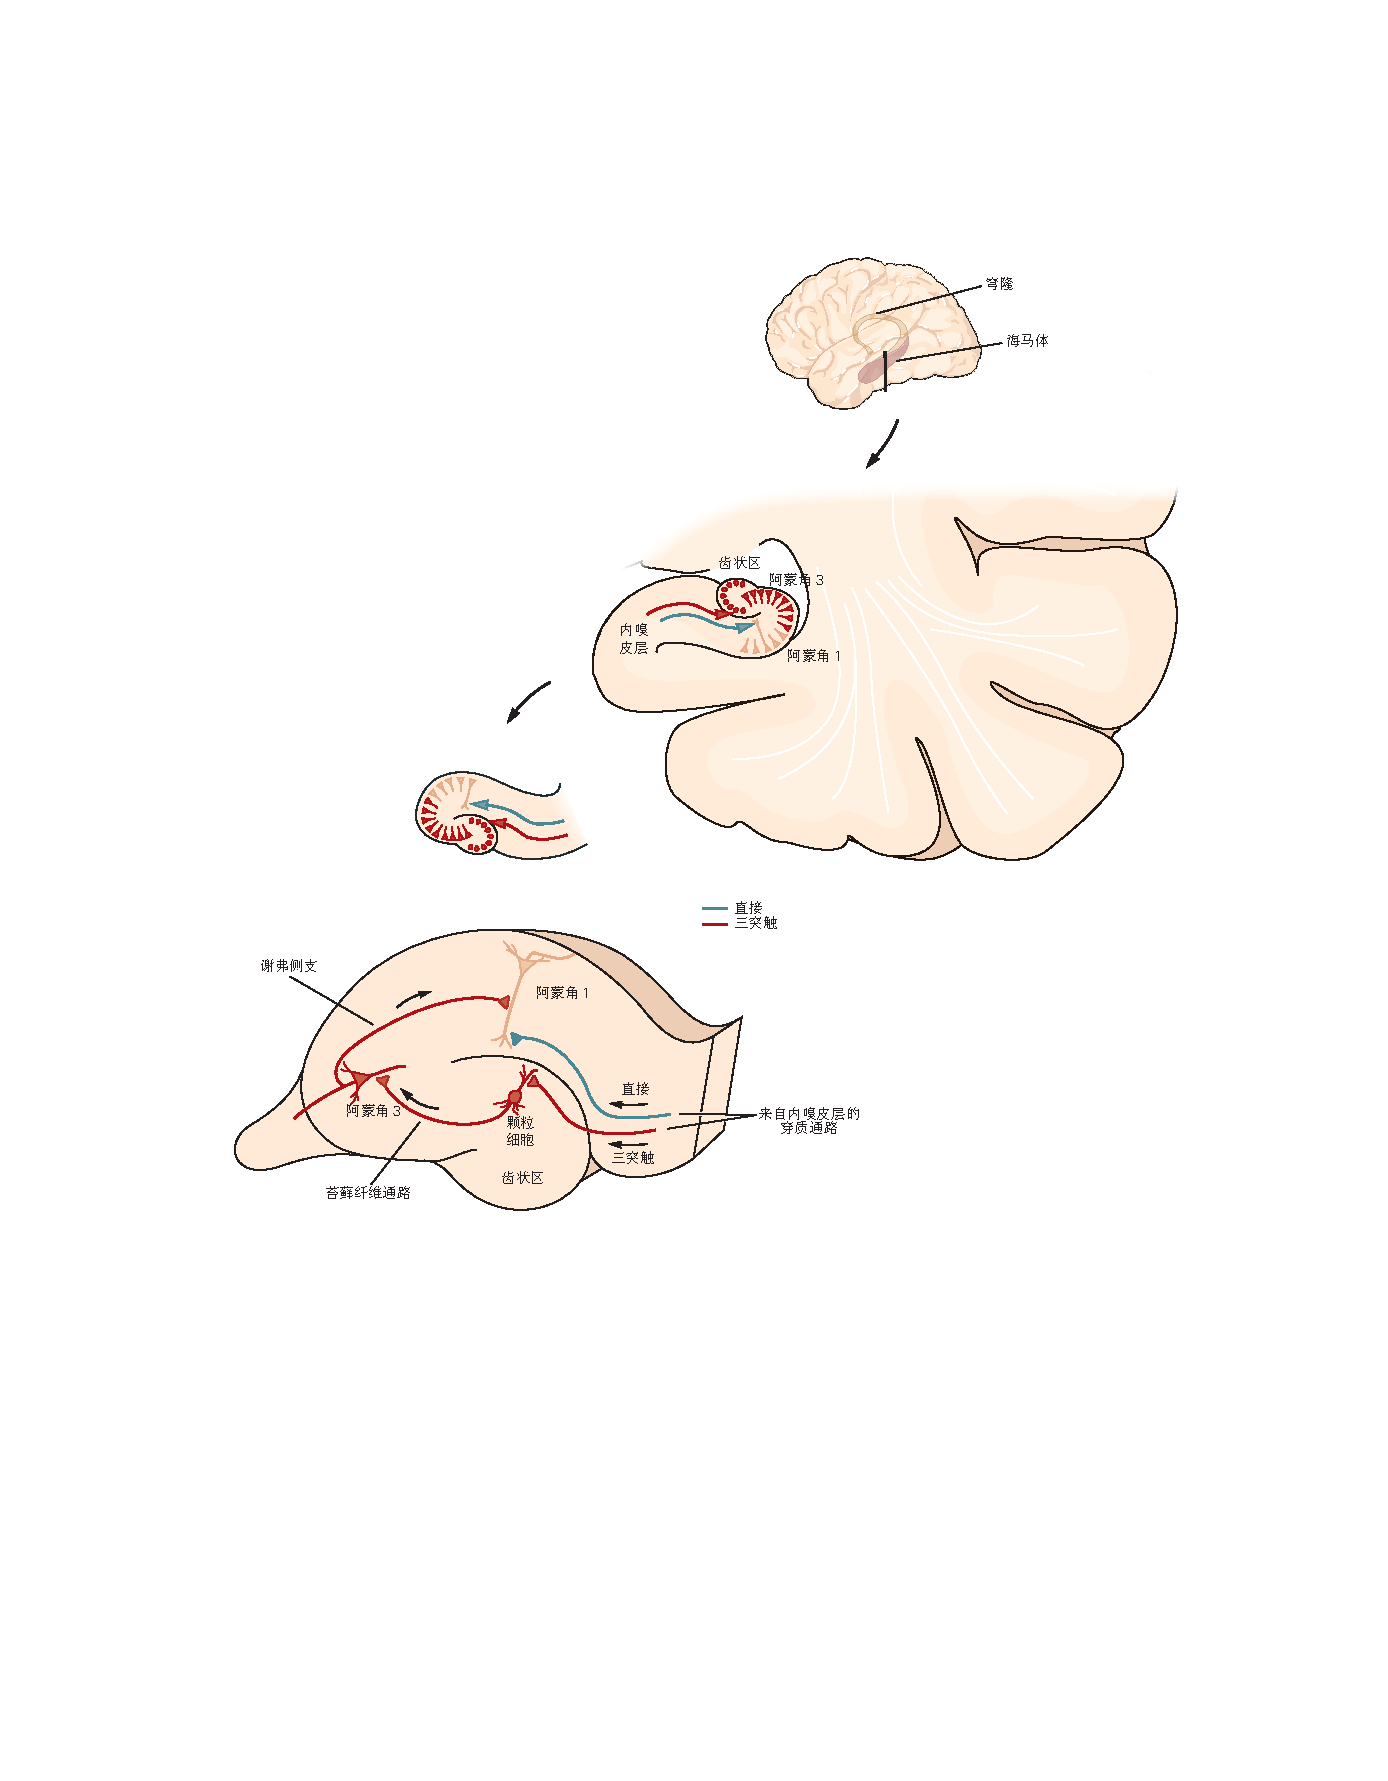
\includegraphics[width=0.9\linewidth]{chap54/fig_54_1}
	\caption{皮质-海马体突触回路对于陈述性记忆很重要。 信息通过穿孔通路从内嗅皮层到达海马体,这些通路为 CA1 区的锥体神经元(海马体的主要输出神经元)提供直接和间接输入。 (箭头表示脉冲流的方向。)间接三突触通路具有三个组件连接。 内嗅皮层 II 层的神经元通过穿孔通路发送它们的轴突,在齿状回的颗粒细胞上形成兴奋性突触。 颗粒细胞通过苔藓纤维通路投射,并与海马 CA3 区的锥体细胞形成兴奋性突触。 CA3 细胞通过 Schaffer 侧支通路刺激 CA1 中的锥体细胞。 在直接通路中,内嗅皮层 III 层的神经元通过穿孔通路投射,在 CA3 和 CA1 锥体神经元的远端树突上形成兴奋性突触,而没有中间突触(仅显示 CA1)。}
	\label{fig:54_1}
\end{figure}


与间接通路并行,内嗅皮层也直接投射到 CA3 和 CA1 海马区域。
在通往 CA1 的直接通路中,内嗅皮层第 III 层中的神经元通过穿孔通路发送其轴突,在 CA1 神经元顶端树突的最远端区域形成兴奋性突触(此类投射也称为颞氨通路)。
海马回路每个阶段的直接和间接输入之间的相互作用可能对记忆存储或回忆很重要,尽管这些相互作用的确切性质仍有待确定。


除了上述连接海马回路不同阶段的通路外,CA3 锥体神经元之间也存在强烈的兴奋性联系。
这种通过循环循环的自激被认为有助于记忆存储和回忆的联想方面。
在病理条件下,这种自激会导致癫痫发作。


最后,位于 CA3 和 CA1 之间的相对较小的 CA2 区域中的神经元通过直接通路和经由齿状回和 CA3 的间接通路从内嗅皮层 II 层接收信息。
CA2 区域还接收来自下丘脑核团的强烈输入,这些核团释放催产素和加压素,这些激素对社会行为很重要。 反过来,CA2 向 CA1 发送强输出,为 CA1 提供第三个兴奋性输入来源(除了来自内嗅皮层的直接和三突触途径)。



\subsection{不同海马通路的长期增强对于外显记忆存储至关重要}

信息如何存储在海马体回路中以提供持久的记忆痕迹?
1973 年,蒂莫西·布利斯 (Timothy Bliss) 和泰耶·洛莫 (Terje Lømo) 发现,短暂的高频突触刺激会导致海马兴奋性突触后电位 (EPSP) 振幅持续增加,这一过程称为长时程增强或 LTP(第 \ref{chap:chap13} 章)。
EPSP 的增强反过来又增加了突触后细胞激发动作电位的可能性。


Bliss 和 Lømo 检查了间接海马通路的初始阶段——由内嗅皮层 II 层神经元与齿状回颗粒神经元的穿孔通路形成的突触。
随后的研究表明,短暂的高频刺激序列可以在该间接通路的几乎所有兴奋性突触以及与 CA3 和 CA1 神经元的直接穿孔通路突触处诱导 LTP 形式(图 \ref{fig:54_2})。
当使用植入电极在完整动物中诱导时,LTP 可以持续数天甚至数周,并且可以在分离的海马体切片和细胞培养物中的海马体神经元中持续数小时。


\begin{figure}[htbp]
	\centering
	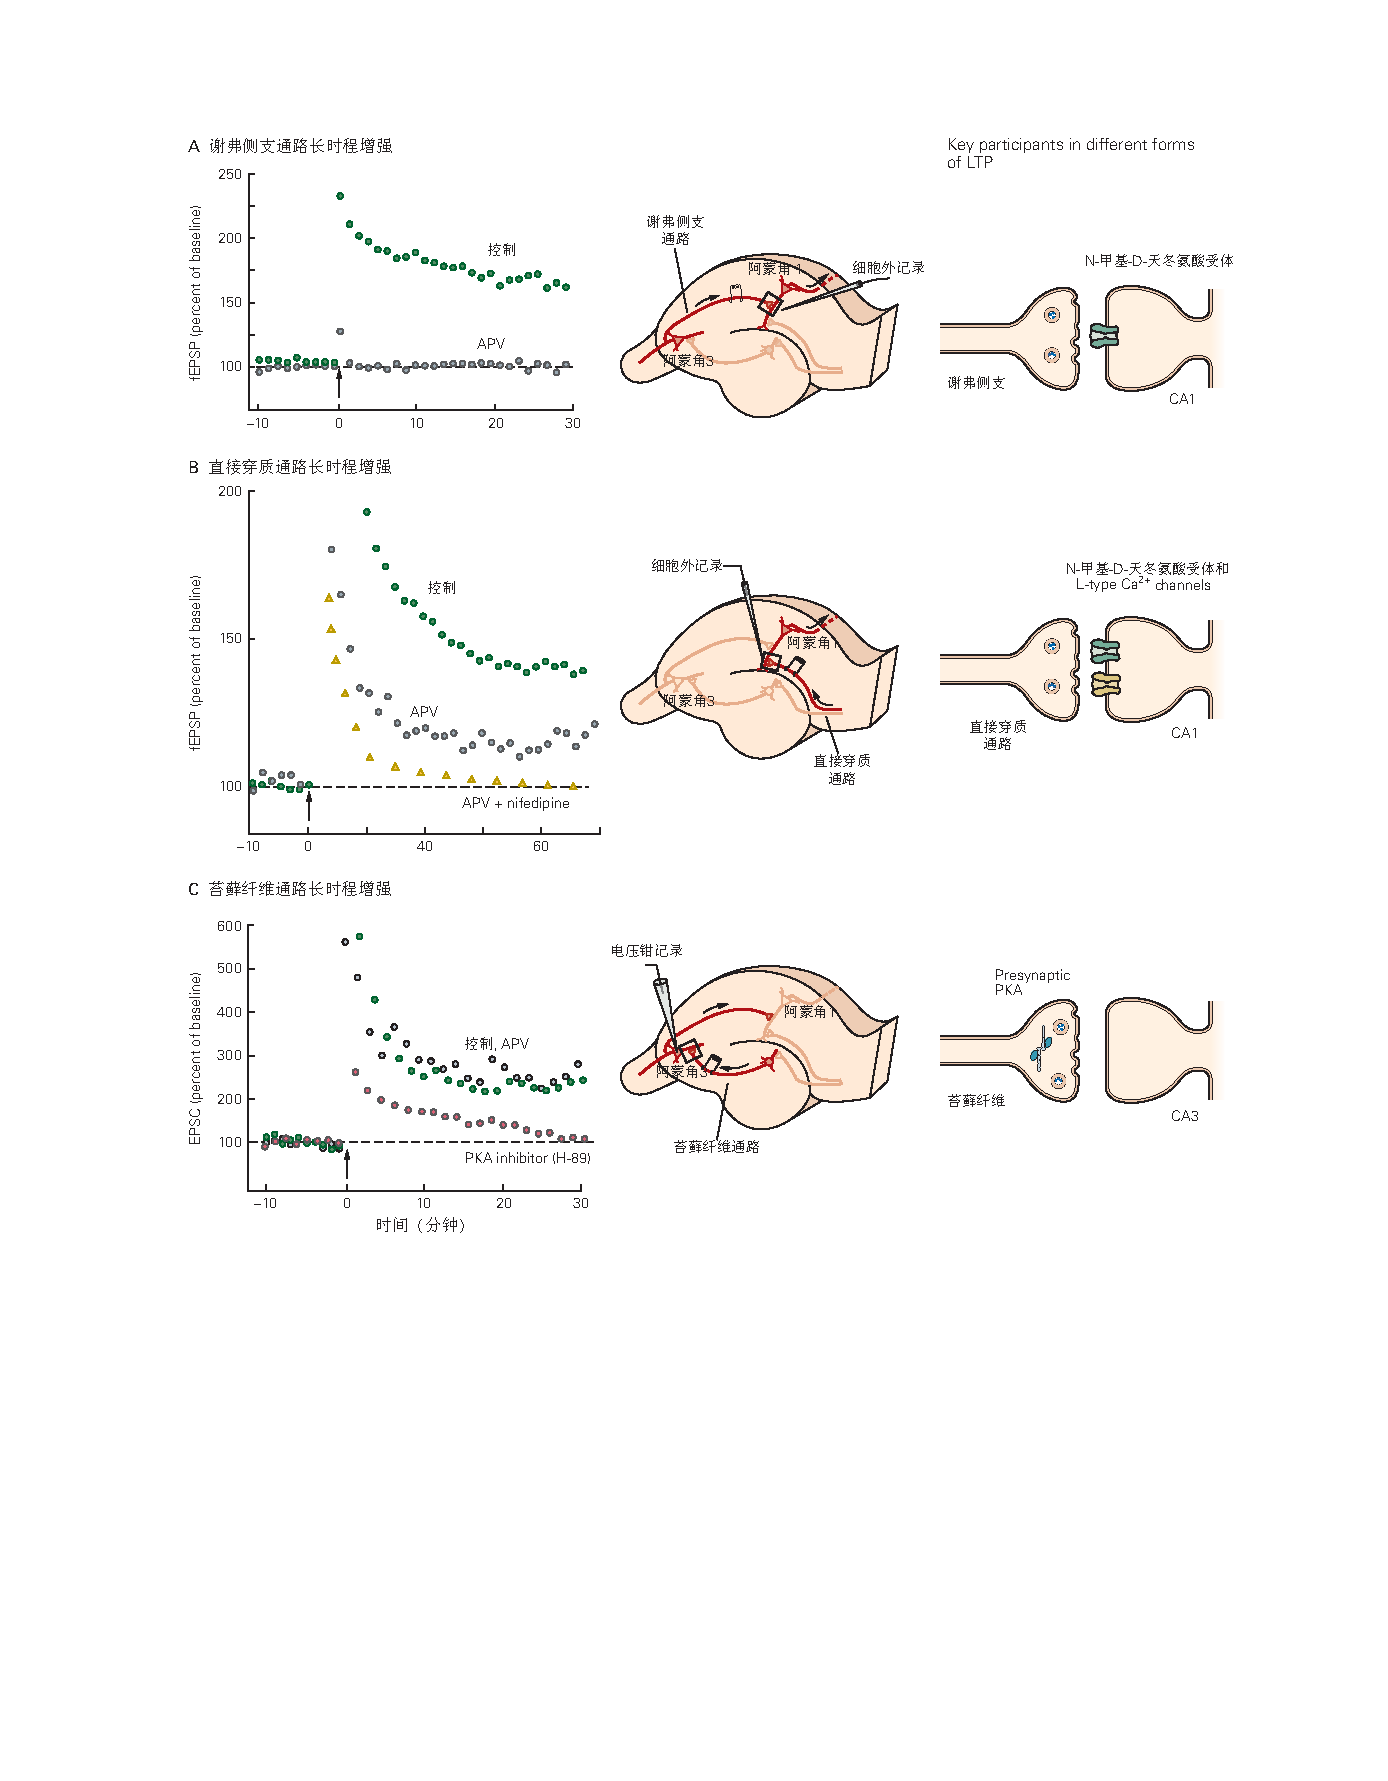
\includegraphics[width=0.9\linewidth]{chap54/fig_54_2}
	\caption{不同的神经机制是三突触通路中三个突触中每一个的长期增强的基础。 长时程增强 (LTP) 发生在整个海马体的突触处,但在不同程度上取决于\textit{N-甲基-D-天冬氨酸}型谷氨酸受体的激活。 A. Schaffer 侧支纤维的破伤风刺激(在图中的时间 0)在突触前 CA3 锥体神经元和突触后 CA1 锥体神经元之间的突触处诱导 LTP。 该图显示细胞外场兴奋性突触后电位 (fEPSP) 的大小占 LTP 诱导前基线 fEPSP 的百分比。 在这些突触处,LTP 需要激活突触后 CA1 神经元中的\textit{N-甲基-D-天冬氨酸}受体通道,因为当破伤风在\textit{N-甲基-D-天冬氨酸}受体拮抗剂 2-氨基-5-膦戊酸 (APV) 存在的情况下被递送时,它被完全阻断。 (改编自 Morgan 和 Teyler 2001。)B. 破伤风刺激从内嗅皮质到 CA1 神经元的直接通路产生 fEPSP 的 LTP,这部分取决于 NMDA 受体通道的激活,部分取决于 L 型电压门控的激活 Ca2+ 通道。 因此它仅被 APV 部分阻断。 需要添加 APV 和硝苯地平,一种阻断 L 型通道的二氢吡啶,以完全抑制 LTP。 C. 破伤风对苔藓纤维通路的刺激在 CA3 区域与锥体细胞的突触处诱导 LTP。 在这个实验中,兴奋性突触后电流 (EPSC) 在电压钳条件下测量。 此 LTP 不需要激活 NMDA 受体,因此不会被 APV 阻断。 然而,它确实需要激活蛋白激酶 A (PKA),因此被激酶抑制剂 H-89 阻断。 (经许可转载自 Zalutsky 和 Nicoll 1990。版权所有 © 1990 AAAS。)}
	\label{fig:54_2}
\end{figure}


对不同海马通路的研究表明,不同突触的 LTP 不是一个单一的过程。
相反,它包含一系列过程,这些过程通过不同的细胞和分子机制加强不同海马突触的突触传递。
事实上,即使在单个突触中,不同形式的 LTP 也可以由不同的突触活动模式诱导,尽管这些不同的过程有许多重要的相似之处。


所有形式的 LTP 都是由正在增强的通路中的突触活动诱导的——也就是说,LTP 是同突触的。
此外,LTP 是突触特异性的;
只有那些被强直刺激激活的突触才会被增强。
然而,不同形式的 LTP 对特定受体和离子通道的依赖性不同。 此外,不同形式的 LTP 募集作用于不同突触位点的不同第二信使信号通路。
一些形式的 LTP 是由对神经递质谷氨酸的突触后反应增强引起的,而其他形式的 LTP 是由突触前末端释放谷氨酸的增强引起的,还有其他形式的 LTP 涉及突触前和突触后神经元。


通过比较 Schaffer 侧支、苔藓纤维和直接内嗅突触的 LTP,可以看出不同形式 LTP 机制的异同。
在所有三种途径中,突触传递持续增强以响应短暂的强直性刺激。
然而,\textit{N-甲基-D-天冬氨酸}受体对 LTP 诱导的贡献在三种途径中有所不同。
在 Schaffer 侧支突触处,当在\textit{N-甲基-D-天冬氨酸}受体拮抗剂 2-氨基-5-膦戊酸(AP5 或 APV)存在的情况下应用破伤风时,LTP 响应于短暂的 100 Hz 刺激的诱导被完全阻断。
相比之下,APV 仅部分抑制在与 CA1 神经元的直接内嗅突触处 LTP 的诱导,并且对在与 CA3 锥体神经元的苔藓纤维突触处的 LTP 没有影响(图 54-2)。


苔藓纤维通路中的长期增强主要是突触前的,由破伤风期间大量 Ca2+ 流入突触前末梢触发。
Ca2+ 流入激活钙/钙调蛋白依赖性腺苷酸环化酶,从而增加环磷酸腺苷 (cAMP) 的产生并激活蛋白激酶 A(PKA;见第 \ref{chap:chap14} 章)。
这导致突触前小泡蛋白磷酸化,从而增强谷氨酸从苔藓纤维末端的释放,从而导致 EPSP 增加。
这种形式的 LTP 不需要突触后细胞的活动。
因此,与赫布可塑性不同,苔藓纤维 LTP 是非关联的。


然而,在 Schaffer 侧支通路中,LTP 是结合的,这主要是由于\textit{N-甲基-D-天冬氨酸}受体的特性(图~\ref{fig:54_3};
另见第 \ref{chap:chap13} 章)。
与大脑中大多数兴奋性突触的情况一样,从 Schaffer 侧支末端释放的谷氨酸激活突触后膜中的 α-amino-3-hydroxy-5-methyl-4-isoxazolepropionic acid (AMPA) 和\textit{N-甲基-D-天冬氨酸}受体通道。
CA1 锥体神经元。 然而,与 AMPA 受体不同,\textit{N-甲基-D-天冬氨酸}受体的激活是相关的,因为它需要同时进行突触前和突触后活动。
这是因为\textit{N-甲基-D-天冬氨酸}受体通道的孔通常在典型的负静息电位下被细胞外 Mg2+ 阻断,这阻止了这些通道响应谷氨酸而传导离子。
为了使\textit{N-甲基-D-天冬氨酸}受体通道有效发挥作用,突触后膜必须充分去极化以通过静电排斥力排出结合的 Mg2+。
以这种方式,\textit{N-甲基-D-天冬氨酸}受体通道充当巧合检测器:
仅当 (1) 突触前神经元中的动作电位释放与受体结合的谷氨酸和 (2) 突触后细胞膜充分去极化时,它才起作用 通过强烈的突触活动来解除 Mg2+ 阻滞。
因此,\textit{N-甲基-D-天冬氨酸}受体能够将突触前和突触后活动联系起来,以募集增强细胞对之间连接的可塑性机制,从而满足 Hebb 对突触修饰的巧合要求。


\begin{figure}[htbp]
	\centering
	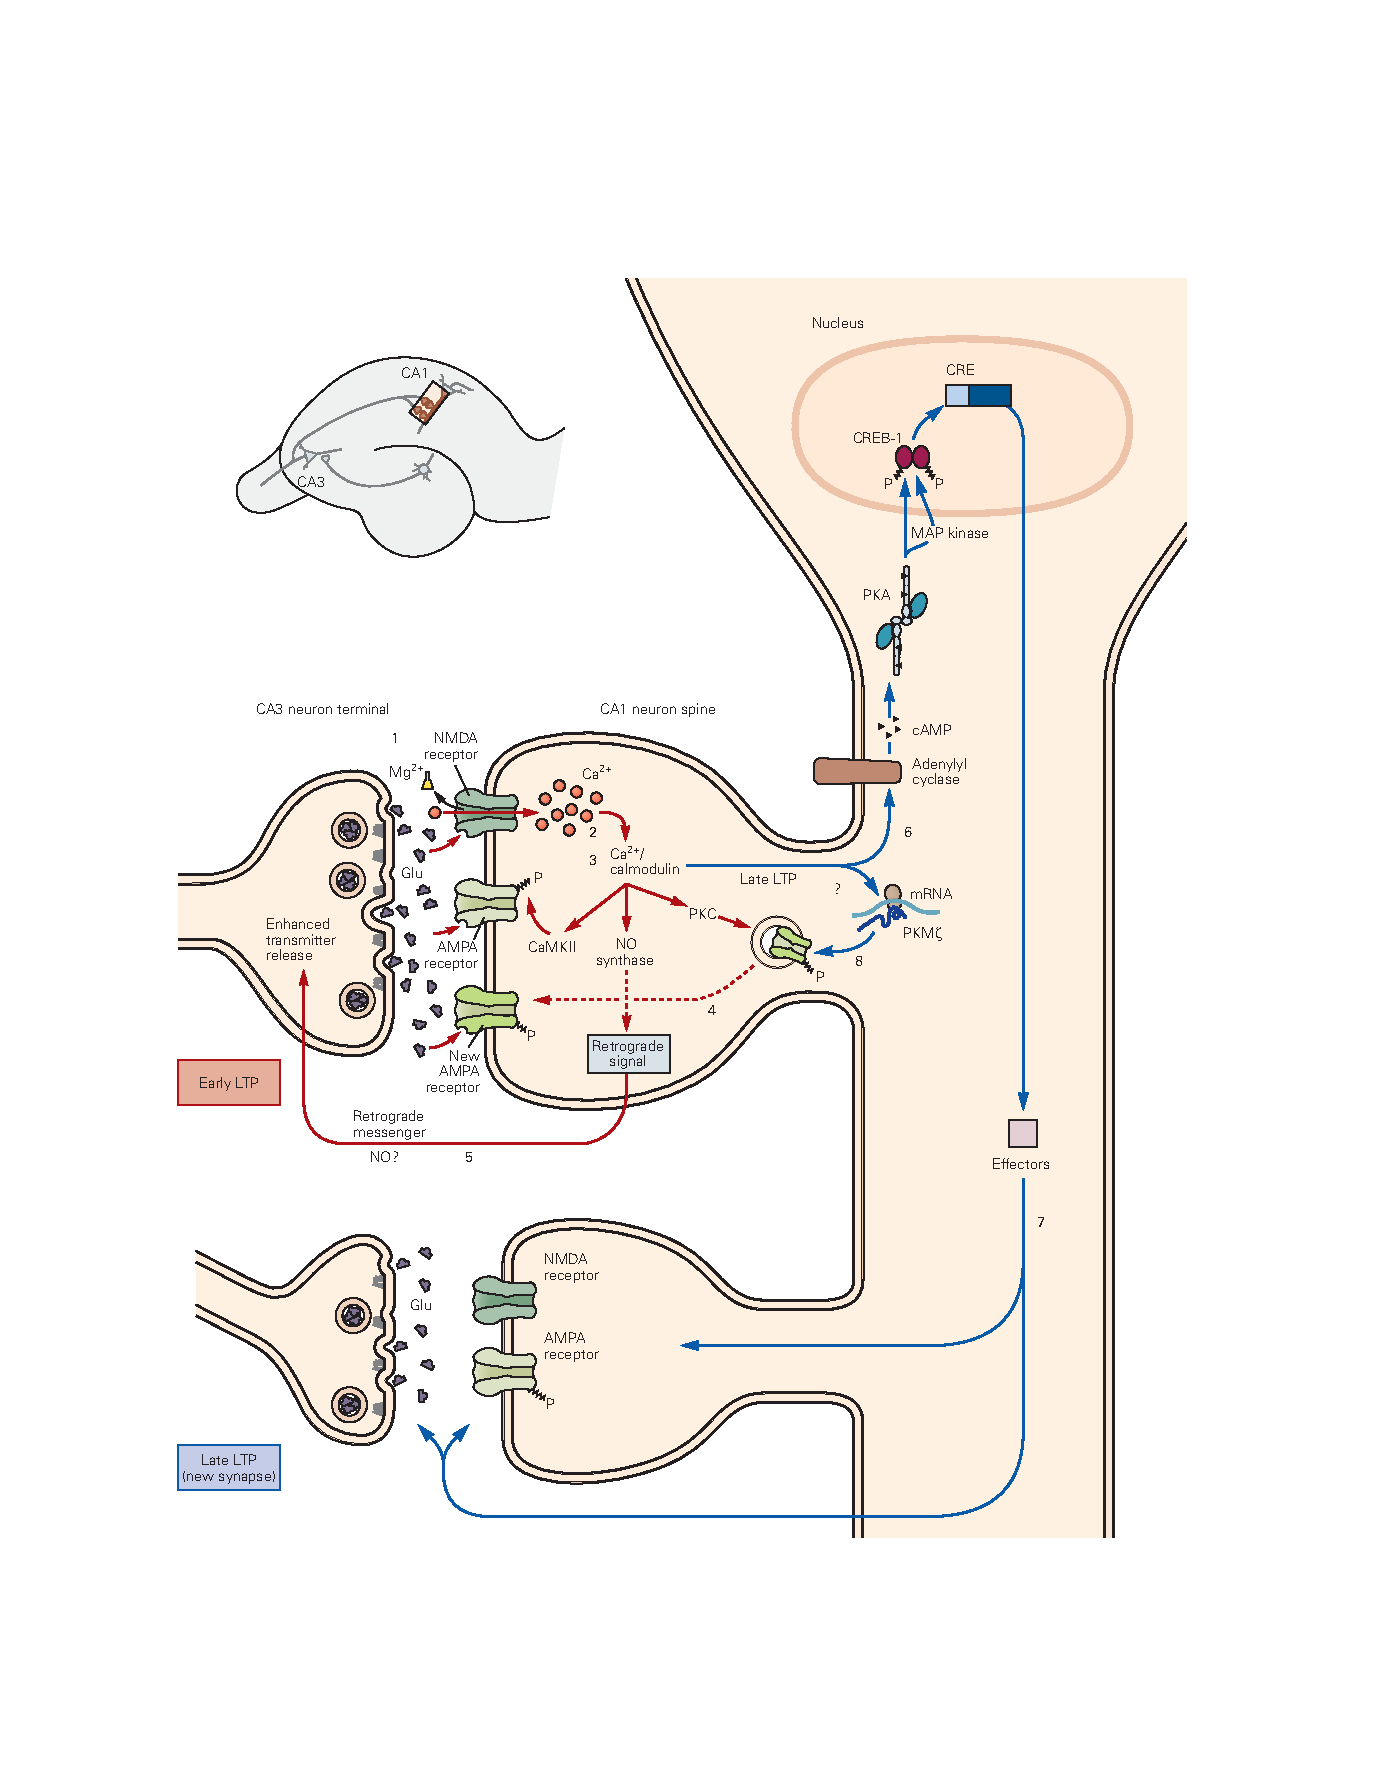
\includegraphics[width=0.9\linewidth]{chap54/fig_54_3}
	\caption{在 Schaffer 侧支突触诱导长期增强 (LTP) 的模型。 一次高频破伤风会诱发早期 LTP。 突触后膜的大量去极化(由 α-amino-3-hydroxy-5-methyl-4-isoxazolepropionic acid [AMPA] 受体的强烈激活引起)减轻了\textit{N-甲基-D-天冬氨酸}的 Mg2+ 阻断 ) 受体通道 (1),允许 Ca2+、Na+ 和 K+ 流过这些通道。 由此导致的树突棘中 Ca2+ 的增加 (2) 触发钙依赖性激酶 (3)——钙/钙调蛋白依赖性激酶 (CaMKII) 和蛋白激酶 C (PKC)——导致 LTP 的诱导。 在诱导 LTP 期间激活的第二信使级联对突触传递有两个主要影响。 通过激活蛋白激酶(包括 PKC)进行的磷酸化增强了通过 AMPA 受体通道的电流,部分原因是导致新受体插入脊柱突触 (4)。 此外,突触后细胞释放逆行信使,如一氧化氮 (NO),激活突触前末梢的蛋白激酶以增强随后的递质释放 (5)。 反复发作的强直刺激会诱发晚期 LTP。 Ca2+ 内流的持续增加会募集腺苷酸环化酶 (6),后者会生成可激活蛋白激酶 A (PKA) 的环磷酸腺苷 (cAMP)。 这导致 MAP 激酶的激活,它转移到细胞核,在那里磷酸化 CREB-1。 CREB-1 反过来激活目标(包含 CRE 启动子)的转录,这些目标被认为会导致新突触连接的生长 (7)。 重复刺激还会激活编码 PKMζ 的\textit{信使核糖核酸}的翻译,PKMζ 是 PKC 的组成型活性亚型 (8)。 这导致突触后膜中 AMPA 受体数量的长期增加。}
	\label{fig:54_3}
\end{figure}


通过强烈的突触兴奋激活\textit{N-甲基-D-天冬氨酸}受体的功能后果是什么?
大多数 AMPA 受体通道仅传导单价阳离子(Na+ 和 K+),而\textit{N-甲基-D-天冬氨酸}受体通道对 Ca2+ 具有高渗透性(第~\ref{chap:chap13} 章)。
因此,这些通道的打开导致突触后细胞中 Ca2+ 浓度的显着增加。
细胞内 Ca2+ 的增加会激活多个下游信号通路,包括钙/钙调蛋白依赖性蛋白激酶 II (CaMKII)、蛋白激酶 C (PKC) 和酪氨酸激酶,从而导致 Schaffer 侧支突触 EPSP 强度增强的变化 (图 \ref{fig:54_3})。



\subsection{不同的分子和细胞机制有助于长期增强的表达形式}

神经科学家经常发现区分 LTP 的诱导(由强直刺激激活的生化反应)和 LTP 的表达(负责增强突触传递的长期变化)是有用的。
在 CA3-CA1 突触处诱导 LTP 的机制主要是突触后的。
LTP 在这个突触中的表达是由递质释放的增加引起的,对固定量递质的突触后反应增加,还是两者的某种组合?


许多实验表明,LTP 的表达形式取决于突触的类型和诱导 LTP 的精确活动模式。
在许多情况下,响应通过\textit{N-甲基-D-天冬氨酸}受体通道的 Ca2+ 流入,CA1 神经元中 LTP 的表达取决于突触后膜对谷氨酸反应的增加。
但是更强的刺激模式可以在同一突触中引发 LTP 的形式,其表达取决于增强递质释放的突触前事件。


突触后对 Schaffer 侧支突触 LTP 表达的贡献的关键证据之一来自对所谓的“沉默突触”的检查。
在一对海马锥体神经元的一些记录中,当一个神经元处于静息电位(约 -70 mV)时,刺激一个神经元的动作电位无法引起突触后神经元的反应。
这个结果并不令人惊讶,因为每个海马突触前神经元只与少数其他神经元相连。
令人惊讶的是,当突触后膜最初处于 –70 mV 时,一些神经元对似乎没有连接,当第二个神经元在电压下去极化时,刺激同一个突触前神经元能够在第二个神经元中引起大的兴奋性突触后电流 钳位到 +30 mV。
在此类神经元对中,突触后膜似乎缺乏功能性 AMPA 受体,因此兴奋性突触后电流 (EPSC) 仅由\textit{N-甲基-D-天冬氨酸}受体通道介导。
因此,当膜保持在细胞的静息电位 (-70 mV) 时,由于这些受体通道的强烈 Mg2+ 阻滞(突触实际上是沉默的),因此没有可测量的 EPSC。
然而,在 +30 mV 时可以生成大的 EPSC,因为去极化解除了阻塞(图 \ref{fig:54_4})。


\begin{figure}[htbp]
	\centering
	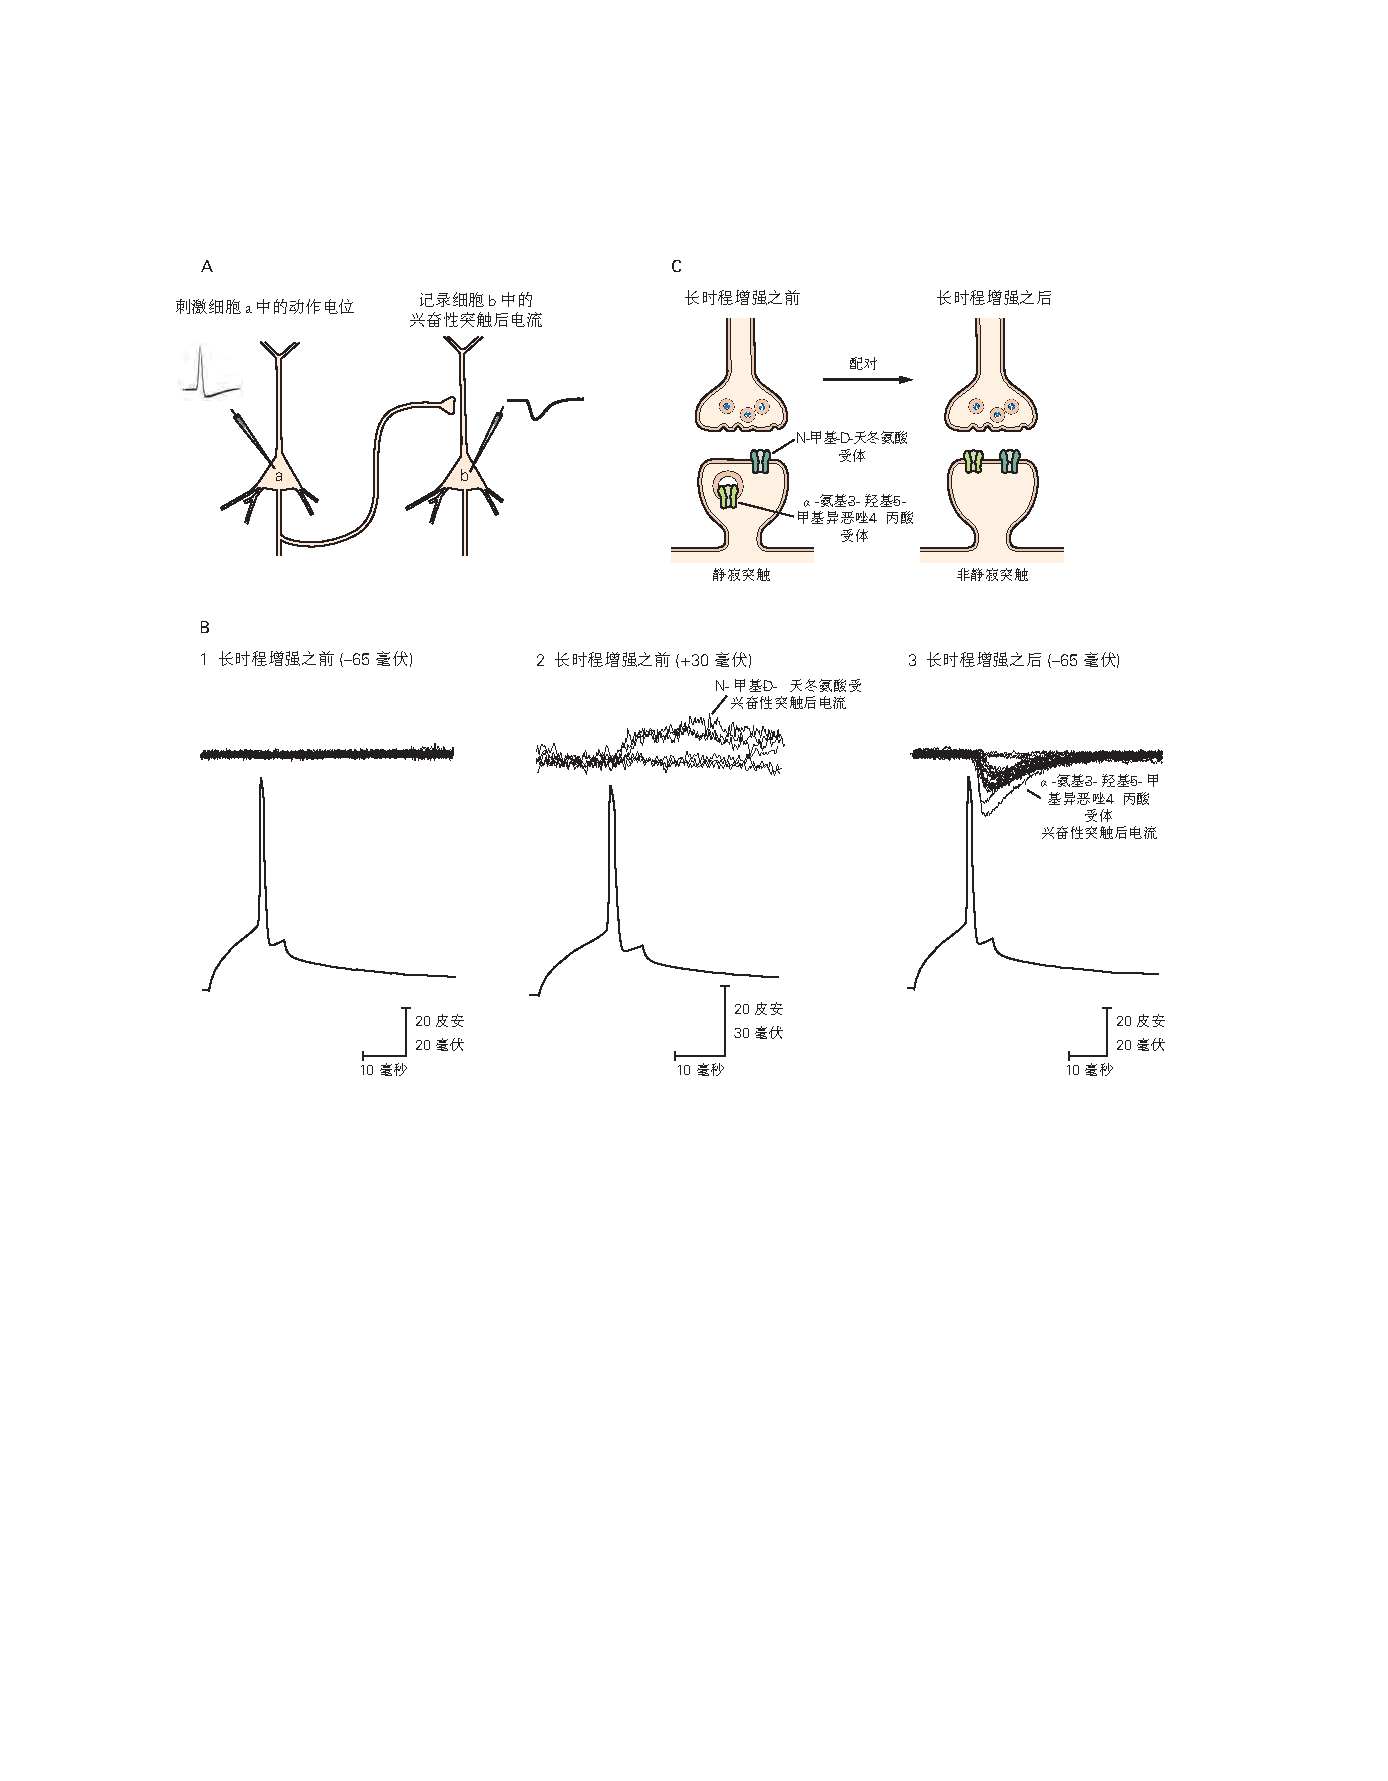
\includegraphics[width=0.85\linewidth]{chap54/fig_54_4}
	\caption{在长时程增强 (LTP) 期间将 α-amino-3-hydroxy-5-methyl-4-isoxazolepropionic acid (AMPA) 受体添加到沉默突触。 A. 细胞内记录是从一对海马锥体神经元中获得的。 去极化电流脉冲在神经元 a 中触发动作电位 (AP),并在电压钳条件下记录神经元 b 中产生的由此产生的兴奋性突触后电流 (EPSC)。 B. 在诱导 LTP 之前,当神经元 b 的膜电位处于其静息值 -65 mV (1) 时,细胞 b 中没有 EPSC(顶部迹线)响应细胞 a 中的动作电位(底部迹线) . 然而,当神经元 b 被电压钳去极化至 +30 mV 时,\textit{N-甲基-D-天冬氨酸}受体被激活,并且观察到这些受体的缓慢 EPSCs 特征 (2)。 然后通过将神经元 a 中的动作电位与神经元 b 中的突触后去极化配对来诱导 LTP,以减轻\textit{N-甲基-D-天冬氨酸}受体的 Mg2+ 阻滞。 配对后,在细胞 b (3) 中可以看到通过激活 AMPA 受体启动的快速 EPSC。 (经许可转载自 Montgomery、Pavlidis 和 Madison 2001。版权所有 © 2001 Cell Press。)C. 沉默突触解除沉默的机制。 在 LTP 之前,突触前 CA3 神经元接触的树突棘仅包含 NMDA 受体。 LTP 诱导后,含有 AMPA 受体的细胞内囊泡在突触处与质膜融合,将 AMPA 受体添加到膜上。}
	\label{fig:54_4}
\end{figure}


在使用强突触刺激诱导 LTP 之后,可以看到这些实验的关键发现。
最初仅由静息突触连接的成对神经元现在通常在负静息电位下表现出大的 EPSP,并且这些 EPSP 由 AMPA 受体介导。
对该结果最简单的解释是,LTP 以某种方式将新的功能性 AMPA 受体募集到沉默的突触膜上,Roberto Malinow 将这一过程称为“AMPAfication”。


LTP 的诱导如何增加 AMPA 受体的反应?
用于诱导 LTP 的强突触刺激会在同一突触后神经元的静默和非静默突触处触发谷氨酸释放。
这导致在非沉默突触处打开大量 AMPA 受体通道,进而产生大量突触后去极化。
然后去极化传播到整个神经元,从而解除 Mg2+ 对非沉默突触和沉默突触的\textit{N-甲基-D-天冬氨酸}受体通道的阻滞。
在静默突触处,通过\textit{N-甲基-D-天冬氨酸}受体通道的 Ca2+ 流入激活生化级联反应,最终导致 AMPA 受体簇插入突触后膜。
这些新插入的 AMPA 受体被认为来自储存在树突棘内体囊泡中的储备池,树突棘是锥体神经元所有兴奋性输入的部位(第 \ref{chap:chap13} 章)。
通过\textit{N-甲基-D-天冬氨酸}受体通道的钙流入提高脊柱 Ca2+ 水平,触发突触后信号级联,导致 PKC 对囊泡 AMPA 受体的细胞质尾部进行磷酸化(第~\ref{chap:chap14} 章),导致它们插入突触后膜(图 54– 3)。


因为几乎所有形式的突触后 LTP 的诱导都需要 Ca2+ 流入突触后细胞,所以在某些形式的 LTP 期间递质释放增强的发现意味着突触前细胞必须从突触后细胞接收到 LTP 已被诱导的信号。
现在有证据表明,突触后细胞中钙激活的第二信使,或者可能是 Ca2+ 本身,导致突触后细胞释放一种或多种化学信使,包括气体一氧化氮,这些化学信使扩散到突触前末梢以增强递质释放(图 \ref{fig:54_3} 和第 \ref{chap:chap14} 章)。
重要的是,这些可扩散的逆行信号似乎只影响那些被强直刺激激活的突触前末梢,从而保持突触特异性。



\subsection{长期增强有早期和晚期}

长时程增强有早期和晚期两个阶段,它们提供了一种调节突触传递增强持续时间的方法。
我们目前关注的阶段仅持续 1 到 3 小时,称为早期 LTP;
该阶段通常由持续 1 秒的 100 Hz 强直刺激的单列引起。
更长时间的活动(使用 3 或 4 组 100 Hz 强直性刺激,每次持续 1 秒)诱导 LTP 的晚期阶段,可以持续 24 小时甚至更长时间。
与早期 LTP 不同,晚期 LTP 需要合成新蛋白质(图 \ref{fig:54_5})。
LTP 的早期阶段是由现有突触的变化介导的,而晚期 LTP 被认为是由成对的共激活神经元之间新的突触连接的生长引起的。


\begin{figure}[htbp]
	\centering
	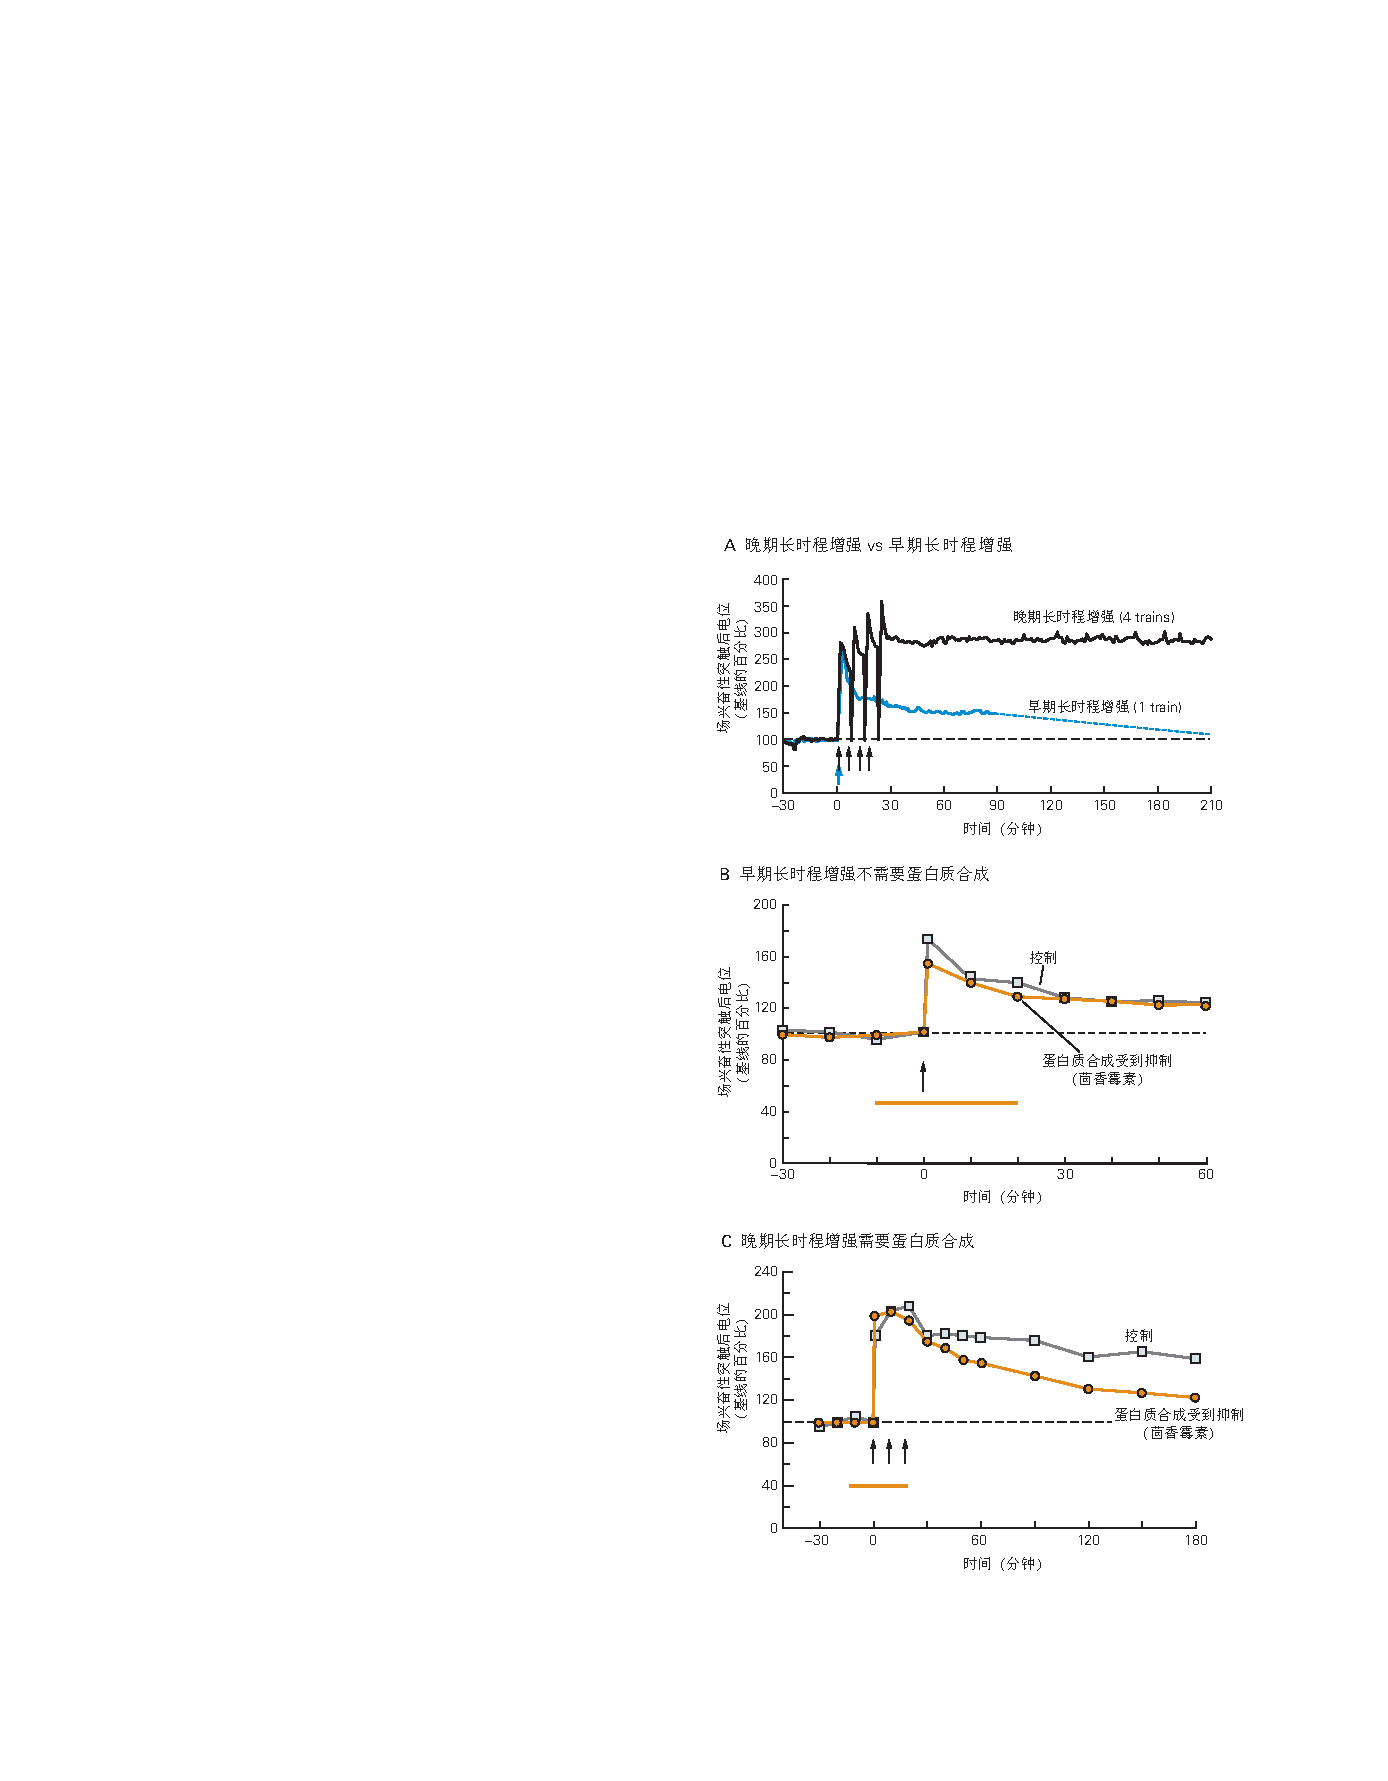
\includegraphics[width=0.5\linewidth]{chap54/fig_54_5}
	\caption{海马 CA1 区的长时程增强 (LTP) 有早期和晚期。 A. 早期 LTP 是由一次破伤风在 100 Hz 下持续 1 秒引起的,而晚期 LTP 是由相隔 10 分钟的四次破伤风引起的。 场兴奋性突触后电位 (fEPSP) 的早期 LTP 仅持续 1 至 2 小时,而晚期 LTP 持续超过 8 小时(仅显示前 3.5 小时)。 B. 一种破伤风引起的早期 LTP 未被蛋白质合成抑制剂茴香霉素 (bar) 阻断。 C. 通常由三列刺激诱导的晚期 LTP 被茴香霉素阻断。 (三或四列火车可用于诱导晚期 LTP。)(B 组和 C 组经许可转载自 Huang 和 Kandel 1994。)}
	\label{fig:54_5}
\end{figure}


尽管 Schaffer 侧支通路和苔藓纤维通路中早期 LTP 的机制完全不同,但两条通路中晚期 LTP 的机制似乎相似(图 \ref{fig:54_3})。
在这两种途径中,晚期 LTP 募集 cAMP 和 PKA 信号通路,通过磷酸化 cAMP 反应元件结合蛋白 (CREB) 转录因子来激活,从而导致新的\textit{信使核糖核酸}和蛋白质的合成。
就像海兔的鳃退缩反射的敏化一样,它也涉及 cAMP、PKA 和 CREB(第 \ref{chap:chap53} 章),Schaffer 侧支通路中的晚期 LTP 是突触特异性的。 当使用间隔一定距离的两个电极刺激同一突触后 CA1 神经元中的两组独立突触时,对一组突触应用四列强直刺激仅在激活的突触处诱导晚期 LTP;
突触传递在第二组未被强直的突触处没有改变。


鉴于转录和大部分翻译发生在细胞体中,晚期 LTP 如何实现突触特异性,这样新合成的蛋白质应该可用于细胞的所有突触?
为了解释突触特异性,Uwe Frey 和 Richard Morris 提出了突触捕获假说,其中在破伤风期间激活的突触以某种方式标记,可能是通过蛋白质磷酸化,这使它们能够利用(“捕获”)新 合成的蛋白质。
Frey 和 Morris 使用上述双路径协议测试了这个想法。
他们在一个电极的一组突触中释放了四个破伤风以诱导晚期 LTP,并在另一个电极的第二组突触中释放了一个破伤风。 虽然单个破伤风自身仅诱发早期 LTP,但在第一个电极出现四次破伤风后 2-3 小时内递送时,它能够诱发晚期 LTP。
这种现象类似于海兔中感觉运动神经元突触的长期易化突触特异性捕获(第 \ref{chap:chap53} 章)。


根据 Frey 和 Morris 的说法,单列破伤风刺激虽然不足以诱导新的蛋白质合成,但足以标记激活的突触,使它们能够捕获新合成的蛋白质,以响应先前传递的四列 强直刺激。
这种标记机制提供的增加的突触可塑性,以及它对新合成蛋白质存在时间的限制,可以解释最近的发现,即存储时间间隔很近的事件记忆的海马细胞集比普通神经元有更多的共同神经元 时间间隔很远的事件的细胞组装。


几个简短的突触刺激序列如何产生如此持久的突触传递增加?
John Lisman 提出的一种机制取决于 CaMKII 的独特属性。
短暂接触 Ca2+ 后,CaMKII 可通过其在苏氨酸 286 (Thr286) 的自磷酸化转化为钙非依赖性状态。
这种响应瞬态 Ca2+ 刺激而变得持续活跃的能力导致了这样的建议,即 CaMKII 可能充当一个简单的分子开关,可以在其初始激活后延长 LTP 的持续时间。


Todd Sacktor 的研究表明,维持晚期 LTP 的更持久变化可能取决于 PKC 的一种非典型亚型,称为 PKMζ (PKM zeta)。
大多数 PKC 亚型都包含一个调节域和一个催化域(第 \ref{chap:chap14} 章)。
二酰基甘油、磷脂和 Ca2+ 与调节域的结合会解除抑制域与催化域的结合,从而使 PKC 磷酸化其蛋白质底物。
相比之下,PKMζ 缺乏调节域,因此具有组成型活性。


海马体中 PKMζ 的水平通常较低。
诱导 LTP 的破伤风刺激通过增强其\textit{信使核糖核酸}的翻译导致 PKMζ 合成的增加。
因为这种\textit{信使核糖核酸}存在于 CA1 神经元树突中,所以它的翻译可以迅速改变突触强度。
在强直刺激期间用肽抑制剂阻断 PKMζ 可阻断晚期 LTP,但不能阻断早期 LTP。
如果阻滞剂在 LTP 诱导后数小时使用,则已建立的晚期 LTP 将被逆转。
这一结果表明,晚期 LTP 的维持需要 PKMζ 的持续活动,以维持突触后膜中 AMPA 受体的增加(图 \ref{fig:54_3})。
在某些条件下,第二种非典型 PKC 亚型可能会替代 PKMζ,这可能解释了 PKMζ 的遗传缺失对晚期 LTP 几乎没有影响这一令人惊讶的发现。


蛋白激酶的组成型活性形式可能不是维持海马体持久突触变化的唯一机制。
重复刺激可能会导致新突触连接的形成,就像海兔在学习过程中长期促进会导致新突触的形成一样。
此外,持久的突触变化可能涉及染色质结构的表观遗传变化。
在晚期 LTP 期间,磷酸化的 CREB 通过招募 CREB 结合蛋白 (CBP) 激活基因表达,CBP 充当组蛋白乙酰化酶,将乙酰基转移到组蛋白上的特定赖氨酸残基,从而产生基因表达的持久变化。
CBP 中的突变会损害小鼠的晚期 LTP 和学习记忆。
在人类中,CBP 基因的从头突变是 Rubinstein-Taybi 综合征的基础,这是一种与智力障碍相关的发育障碍。
其他研究表明第二种表观遗传机制,即\textit{脱氧核糖核酸}甲基化,与持久的突触可塑性和学习记忆有关。



\subsection{尖峰时间依赖性可塑性为改变突触强度提供了更自然的机制}

在大多数情况下,海马神经元不会产生通常用于通过实验诱导 LTP 的高频动作电位序列。
然而,一种称为尖峰时间依赖性可塑性 (STDP) 的 LTP 形式可以通过更自然的活动模式诱导,其中单个突触前刺激与突触后细胞中相对较低的单个动作电位的发射配对 频率(例如,在几秒钟内每秒一对)。
然而,突触前细胞必须在突触后细胞之前发射。 相反,如果突触后细胞恰好在 EPSP 之前发射,则 EPSP 的大小会出现长期下降。
这种突触传递的长期抑制代表了与 LTP 不同的突触可塑性形式,下文将对此进行更全面的描述。
如果突触后动作电位发生在 EPSP 之前或之后一百毫秒以上,则突触强度不会发生变化。


因此,STDP 的配对规则遵循 Hebb 的假设,并在很大程度上源于\textit{N-甲基-D-天冬氨酸}受体通道的协同特性。
如果突触后尖峰发生在 EPSP 期间,它能够在\textit{N-甲基-D-天冬氨酸}受体被谷氨酸结合激活时解除通道的 Mg2+ 封锁。
这导致大量 Ca2+ 通过受体流入并诱导 STDP。
然而,如果突触后动作电位发生在谷氨酸的突触前释放之前,则当受体通道的门关闭时(因为没有谷氨酸),Mg2+ 阻滞的任何释放都会发生。
结果,只有少量 Ca2+ 流入受体,不足以诱导 STDP。



\subsection{海马体中的长期增强具有使其可用作记忆存储机制的特性}

Schaffer 侧支通路和其他海马通路中的\textit{N-甲基-D-天冬氨酸}受体依赖性 LTP 具有三个与学习和记忆直接相关的特性(图~\ref{fig:54_6})。
首先,此类通路中的 LTP 需要几乎同时激活大量传入输入,这一特征称为协同性(图 \ref{fig:54_6})。
这一要求源于这样一个事实,即\textit{N-甲基-D-天冬氨酸}受体通道的 Mg2+ 阻滞的缓解需要大量去极化,这只有在突触后细胞接收来自大量突触前细胞的输入时才能实现。


\begin{figure}[htbp]
	\centering
	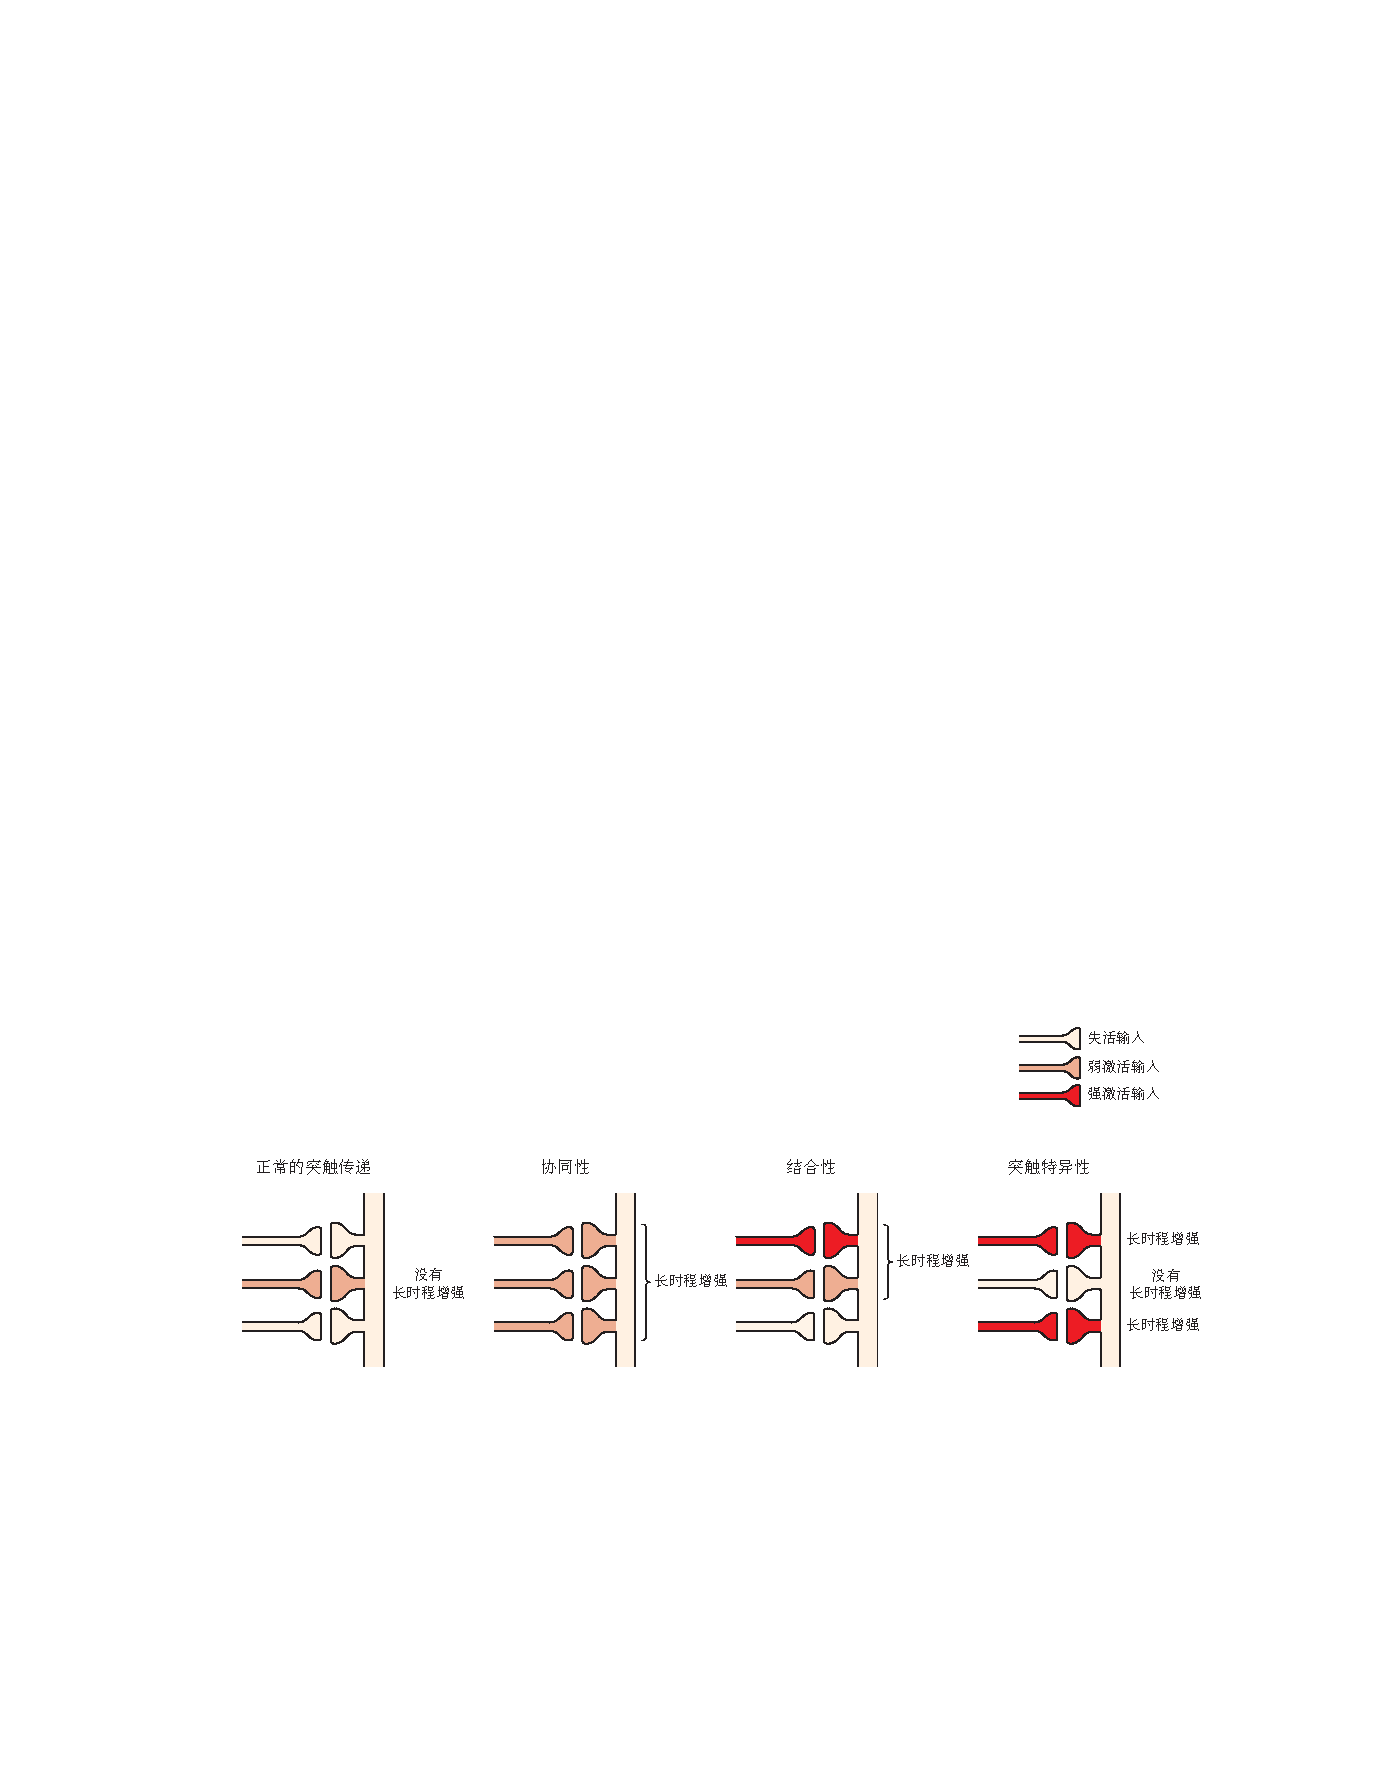
\includegraphics[width=0.9\linewidth]{chap54/fig_54_6}
	\caption{海马 CA1 锥体神经元的长时程增强 (LTP) 表现出协同性、结合性和突触特异性。 在正常突触传递的情况下,一个或几个轴突中的单一动作电位(弱输入)导致小的兴奋性突触后电位(EPSP)不足以从\textit{N-甲基-D-天冬氨酸}受体通道中排出 Mg2+,因此 不能诱导 LTP。 这确保了不相关的刺激不会被记住。 在强激活(协同)过程中,几个弱输入的几乎同时激活会产生超阈值 EPSP,触发动作电位,从而在所有通路中产生 LTP。 同时刺激强输入和弱输入(关联性)会导致两种途径中的 LTP。 通过这种方式,当与强大的输入配对时,弱输入变得重要。 尽管相邻突触受到强烈刺激,但未受刺激的突触不会经历 LTP。 这确保了记忆被选择性地存储在活跃的突触中(突触特异性)。}
	\label{fig:54_6}
\end{figure}


其次,与\textit{N-甲基-D-天冬氨酸}受体通道突触处的 LTP 是关联的。
弱的突触前输入通常不会产生足够的突触后去极化来诱导 LTP。
然而,如果弱输入与产生超阈值去极化的强输入配对,则由此产生的大去极化将传播到具有弱输入的突触,导致\textit{N-甲基-D-天冬氨酸}受体的 Mg2+ 阻断解除并在这些突触处诱导 LTP。


第三,\textit{N-甲基-D-天冬氨酸}受体依赖性 LTP 是突触特异性的。
如果在强烈的突触刺激期间未激活特定突触,则该位点的\textit{N-甲基-D-天冬氨酸}受体将无法结合谷氨酸,因此尽管有强烈的突触后去极化也不会被激活。
因此,该突触不会经历 LTP。


这三个属性(协同性、关联性和突触特异性)中的每一个都是记忆存储的关键要求。
协同性确保只有高度重要的事件,即激活足够输入的事件,才会导致记忆存储。
联想性,如联想巴甫洛夫条件反射,允许一个本身意义不大的事件(或条件刺激)被赋予更高程度的意义,如果该事件发生在另一个更重要的事件(无条件刺激)之前或同时发生的话。
在具有强循环连接的网络中,例如 CA3,关联 LTP 使一组细胞中的活动模式与独立但部分重叠的一组突触耦合细胞中的不同活动模式相关联。
细胞集合的这种联系被认为可以使相关事件相互关联,并且对于存储和回忆大量经验非常重要,就像外显记忆一样。
最后,突触特异性确保传递与特定事件无关的信息的输入不会被加强。
当大量信息必须存储在一个网络中时,突触特异性是至关重要的,因为通过单个突触的功能改变可以在细胞中存储更多信息,而不是通过细胞特性(如兴奋性)的全面变化来存储。



\subsection{空间记忆取决于长期增强}

长时程增强是一种实验诱导的突触强度变化,由对神经通路的强烈直接刺激产生。
这种或相关形式的突触可塑性是否在外显记忆存储期间在生理上发生?
如果是这样,海马体中的外显记忆存储有多重要?


迄今为止,大量实验方法表明抑制 LTP 会干扰空间记忆。
在一种方法中,将老鼠放在充满不透明液体的水池中(Morris 水迷宫);
为了逃离液体,老鼠必须游到一个淹没在液体中并且完全看不见的平台。
该动物在泳池周围的随机位置被释放,最初偶然遇到平台。
然而,在随后的试验中,老鼠很快学会定位平台,然后根据空间信息记住它的位置——水池所在房间墙壁上的远端标记。
这个任务需要海马体。
在此测试的非空间或提示版本中,平台升高到水面以上或标有旗帜以使其可见,从而允许小鼠使用不需要海马体的大脑通路直接导航到它。


当\textit{N-甲基-D-天冬氨酸}受体在动物接受 Morris 水迷宫导航训练之前立即被注入海马体的药理学拮抗剂阻断时,动物无法使用空间信息记住隐藏平台的位置,但可以在任务版本中找到它 可见标记。
因此,这些实验表明,涉及海马体中\textit{N-甲基-D-天冬氨酸}受体的某些机制,可能是 LTP,参与了空间学习。
然而,如果在动物学习空间记忆任务后将\textit{N-甲基-D-天冬氨酸}受体阻滞剂注射到海马体中,它不会抑制随后对该任务的记忆回忆。
这与诱导而非维持 LTP 需要\textit{N-甲基-D-天冬氨酸}受体的发现一致。


与记忆形成和 LTP 相关的更直接证据来自对具有干扰 LTP 的遗传损伤的突变小鼠的实验。
一个有趣的突变是由\textit{N-甲基-D-天冬氨酸}受体的 NR1 亚基基因缺失引起的。
缺少该亚基的神经元无法形成功能性\textit{N-甲基-D-天冬氨酸}受体。
一般缺失该亚基的小鼠在出生后不久就会死亡,表明这些受体对神经功能的重要性。
然而,有可能产生条件突变小鼠系,其中 NR1 缺失仅限于 CA1 锥体神经元,并且仅在出生后 1 或 2 周发生(参见第 \ref{chap:chap2} 章,图 2-8,了解该小鼠系如何 生成)。
这些小鼠存活到成年期,并在 Schaffer 侧支通路中显示 LTP 丢失。
尽管这种破坏是高度局部化的,但突变小鼠的空间记忆存在严重缺陷(图 \ref{fig:54_7})。


\begin{figure}[htbp]
	\centering
	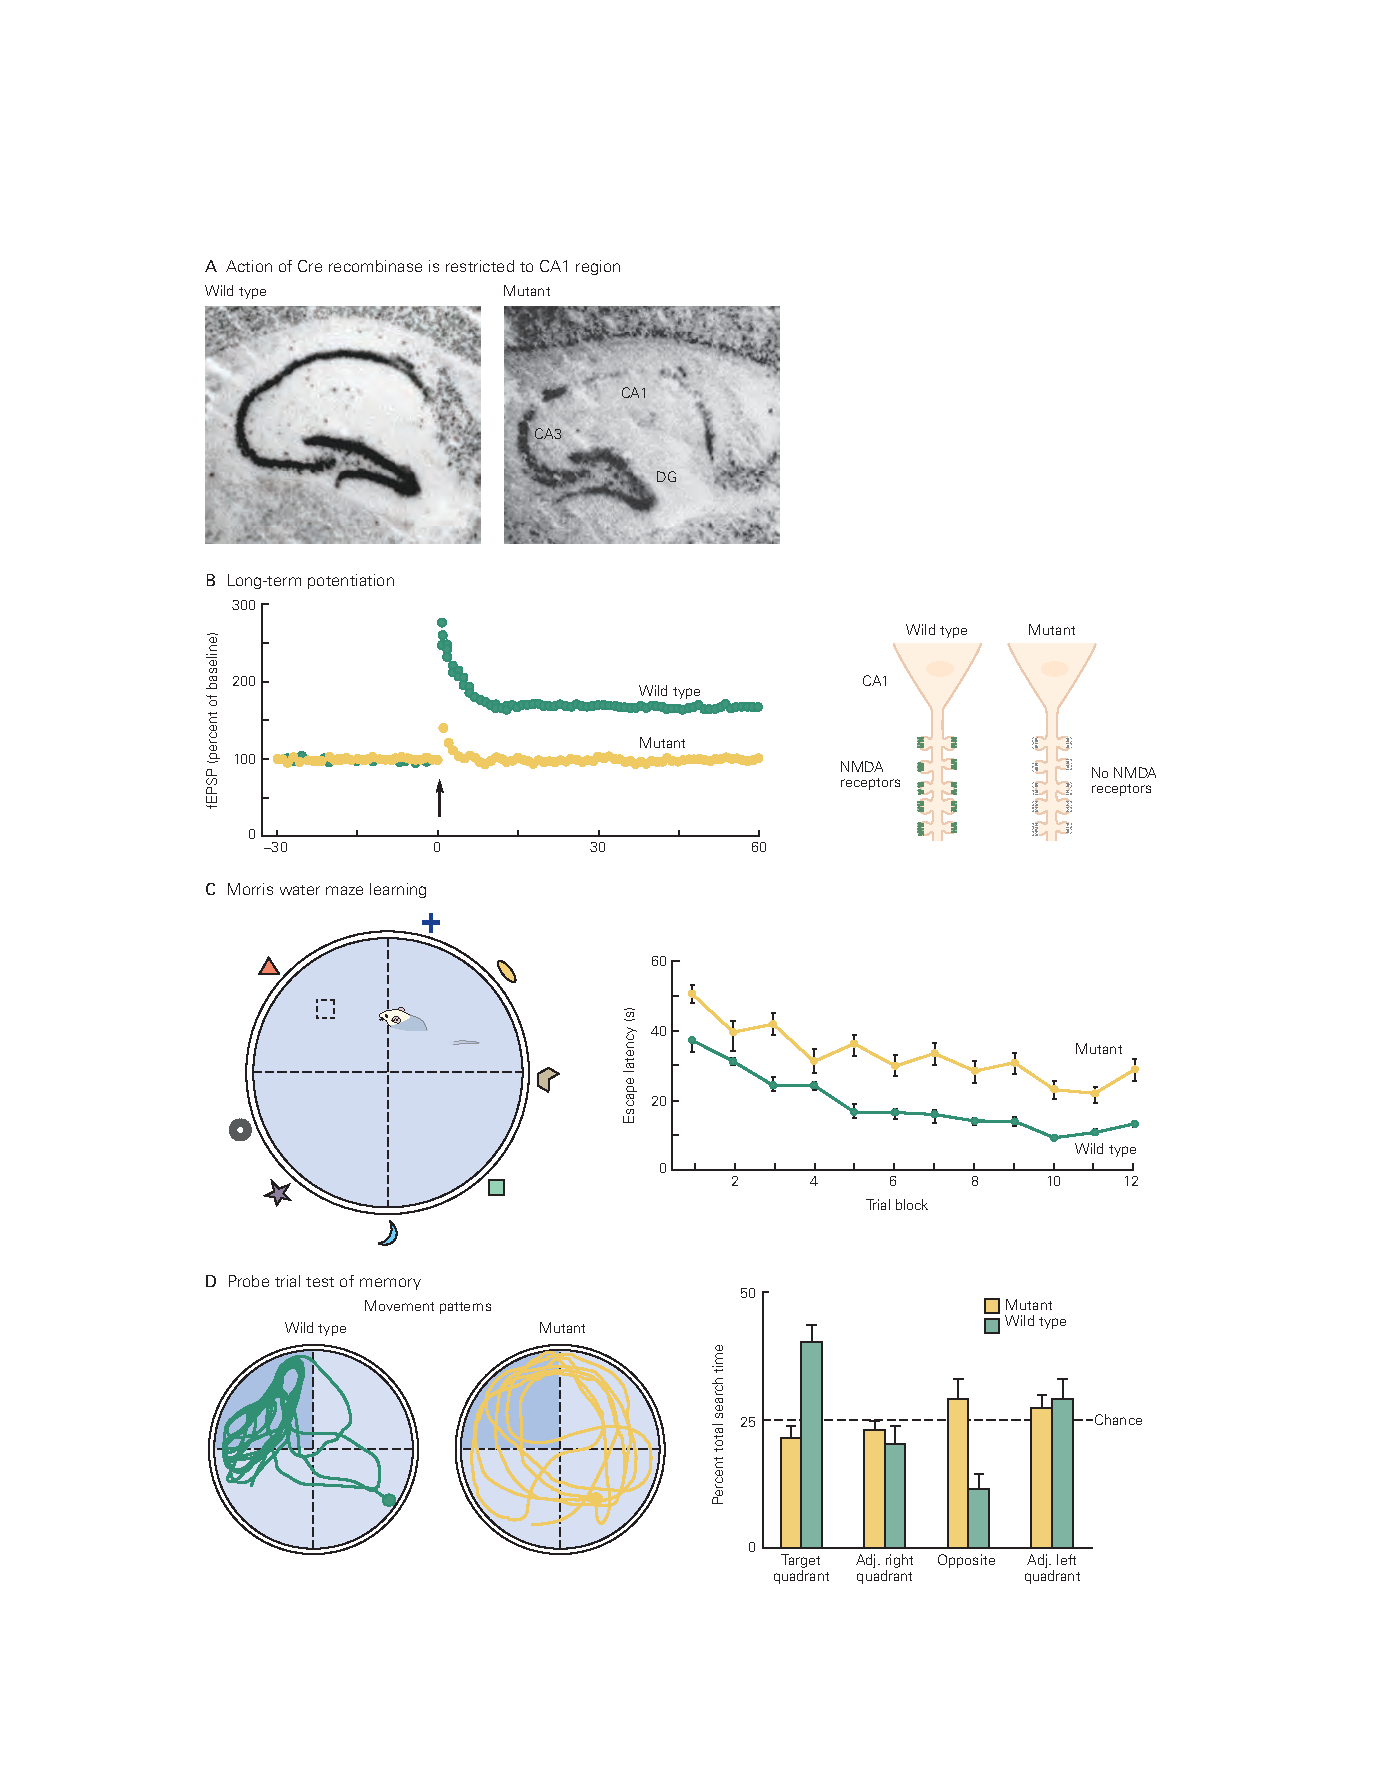
\includegraphics[width=0.9\linewidth]{chap54/fig_54_7}
	\caption{在海马体 CA1 区域缺乏\textit{N-甲基-D-天冬氨酸}受体的小鼠中,长时程增强 (LTP) 和空间学习和记忆受损。 (经许可转载自 Tsien、Huerta 和 Tonegawa 1996。) A. 培育了一系列小鼠,其中编码 NMDA 受体的 NR1 亚基的基因在 CA1 锥体神经元中被选择性删除。 原位杂交用于检测野生型和突变小鼠海马切片中 NR1 亚基的\textit{信使核糖核酸},这些小鼠含有两个 floxed NR1 等位基因,并在 CaMKIIα 启动子的控制下表达 Cre 重组酶。 请注意,NR1 mRNA 表达(深色染色)在海马体的 CA1 区域大大减少,但在 CA3 和齿状回 (DG) 中没有。 B. 在这些小鼠中,CA1 Schaffer 侧支突触的 LTP 被废除。 场兴奋性突触后电位 (fEPSPs) 被记录为对 Schaffer 侧支刺激的反应。 在 100 Hz 下持续 1 秒(箭头)的破伤风刺激在野生型小鼠中引起大幅增强,但未能在 NMDA 受体敲除(突变)小鼠中诱导 LTP。 C. 在 CA1 锥体神经元中缺乏 NMDA 受体的小鼠空间记忆受损。 平台(虚线方块)浸没在圆形水箱(Morris 水迷宫)中的不透明液体中。 为了避免留在水中,老鼠必须使用水箱周围墙壁上的空间(上下文)线索找到平台,然后爬上平台。 该图显示了逃逸潜伏期或小鼠在连续试验中找到隐藏平台所需的时间。 与野生型小鼠相比,突变小鼠在每个试验组(每天四次试验)中表现出更长的逃避潜伏期。 此外,经过 12 天的训练后,突变小鼠并没有达到对照小鼠所达到的最佳性能,尽管它们在训练后表现出一些改善。 D. 小鼠在 Morris 迷宫中训练完成后,平台被拿走。 在这个探测试验中,野生型小鼠在以前包含平台的象限(目标象限)中花费了不成比例的时间,表明它们记住了平台的位置。 突变小鼠在所有象限中花费的时间相同 (25\%); 也就是说,他们的表现是偶然的,表明记忆力不足。}
	\label{fig:54_7}
\end{figure}


在某些情况下,基因变化实际上可以增强海马 LTP 和空间学习和记忆。
这种增强的第一个例子来自对过度表达\textit{N-甲基-D-天冬氨酸}受体的 NR2B 亚基的突变小鼠的研究。
该亚基通常存在于发育早期的海马突触中,但在成人中下调。
包含该亚基的受体比不含该亚基的受体允许更多的 Ca2+ 流入。
在过度表达 NR2B 亚基的突变小鼠中,LTP 增强,可能是因为 Ca2+ 流入增强。
重要的是,几个不同任务的学习和记忆也得到了增强(图 \ref{fig:54_8})。


\begin{figure}[htbp]
	\centering
	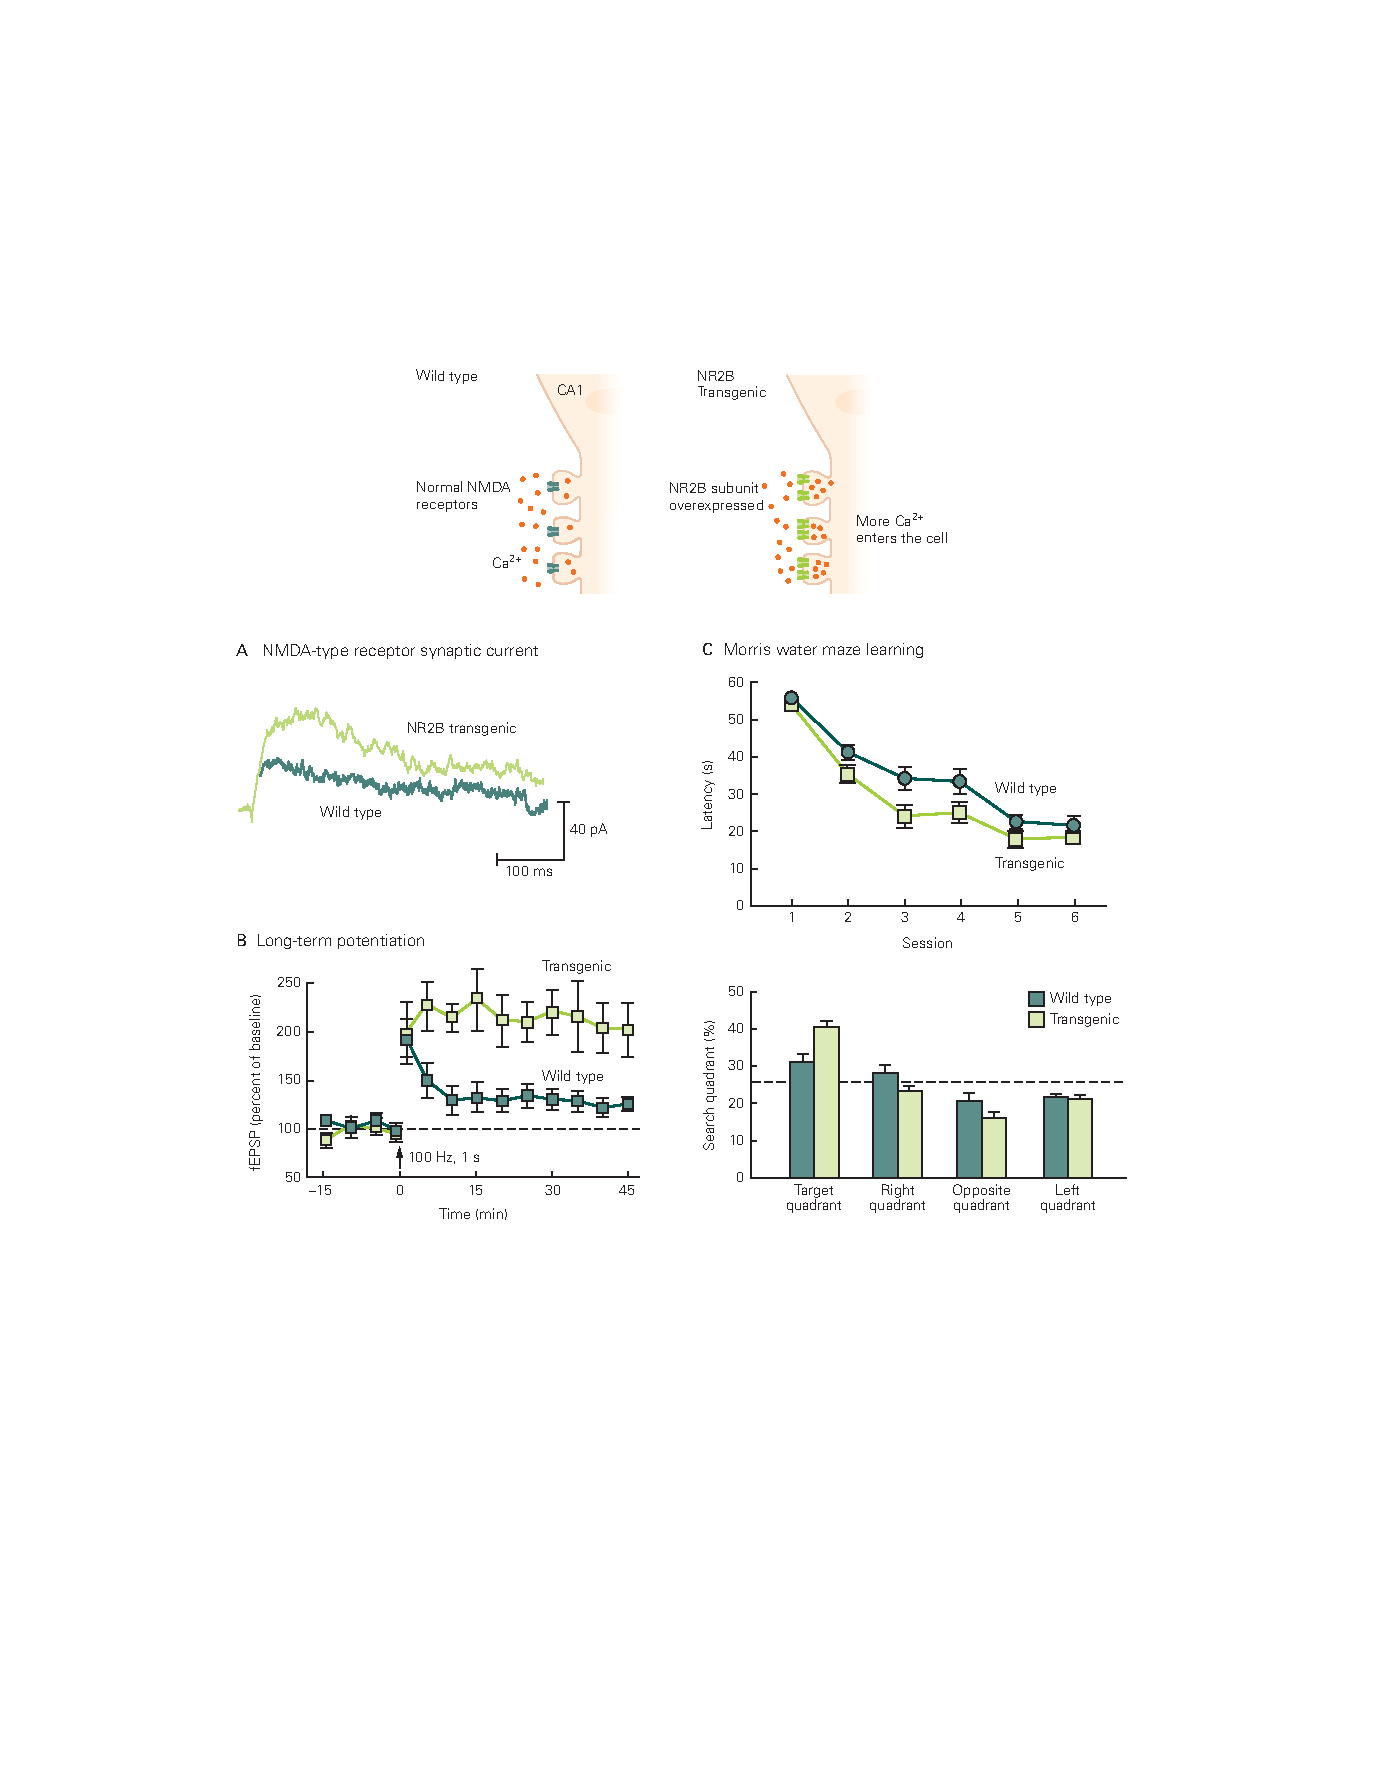
\includegraphics[width=0.75\linewidth]{chap54/fig_54_8}
	\caption{过度表达\textit{N-甲基-D-天冬氨酸}谷氨酸受体亚基的小鼠的学习和记忆得到增强。 (经许可转载自 Tang et al. 1999。版权所有 © 1999 Springer Nature。) A. \textit{N-甲基-D-天冬氨酸}受体响应谷氨酸的短暂脉冲而产生的电流振幅增强,其在海马神经元中的时程延长 从含有转基因的小鼠中获得,与野生型小鼠相比,该转基因表达更高水平的受体 NR2B 亚基。 B. 强直刺激 Schaffer 侧支突触产生的长时程增强在转基因小鼠中比在野生型小鼠中更大。 (缩写:fEPSP,场兴奋性突触后电位。)C. 转基因小鼠的空间学习得到增强(上图)。 转基因小鼠在莫里斯水迷宫中的学习速度(减少寻找隐藏平台的时间,或逃避潜伏期)比野生型小鼠更快。 转基因小鼠的空间记忆也得到增强(下图)。 在探测试验中,转基因小鼠比野生型小鼠在目标象限中停留的时间更长,该象限之前包含隐藏平台。}
	\label{fig:54_8}
\end{figure}


基因敲除或转基因表达的一个担忧是,此类突变可能会导致细微的发育异常。
也就是说,突变动物 LTP 和空间记忆大小的变化可能是海马回路线路早期发育改变的结果,而不是 LTP 基本机制的变化。
这种可能性可以通过可逆地打开和关闭干扰 LTP 的转基因来解决。


可逆基因表达已被用于探索 CaMKII 的作用,其自磷酸化特性和在 LTP 中的功能已在本章前面讨论过(另请参见第 \ref{chap:chap2} 章图 2-9,了解该方法的描述)。
自磷酸化 Thr286 位点突变为带负电荷的氨基酸天冬氨酸模拟 Thr286 自磷酸化的作用并将 CaMKII 转化为钙非依赖性形式。
这种 CaMKII 显性突变 (CaMKII-Asp286) 的转基因表达导致破伤风频率与长期可塑性期间突触强度由此产生的变化之间的关系发生系统性转变。


在转基因小鼠中,中频 10 赫兹的破伤风刺激(通常会诱导少量 LTP)会导致 Schaffer 侧支通路中突触传递的长期抑制(图 \ref{fig:54_9}A)。
相反,转基因小鼠对 100 Hz 破伤风表现出正常的 LTP。 10 赫兹刺激的突触可塑性缺陷与突变小鼠无法记住空间任务有关。
然而,当突变基因在成人中关闭时,LTP 诱导和空间记忆的缺陷可以完全消失,表明记忆缺陷不是由于发育异常引起的(图 \ref{fig:54_9})。


\begin{figure}[htbp]
	\centering
	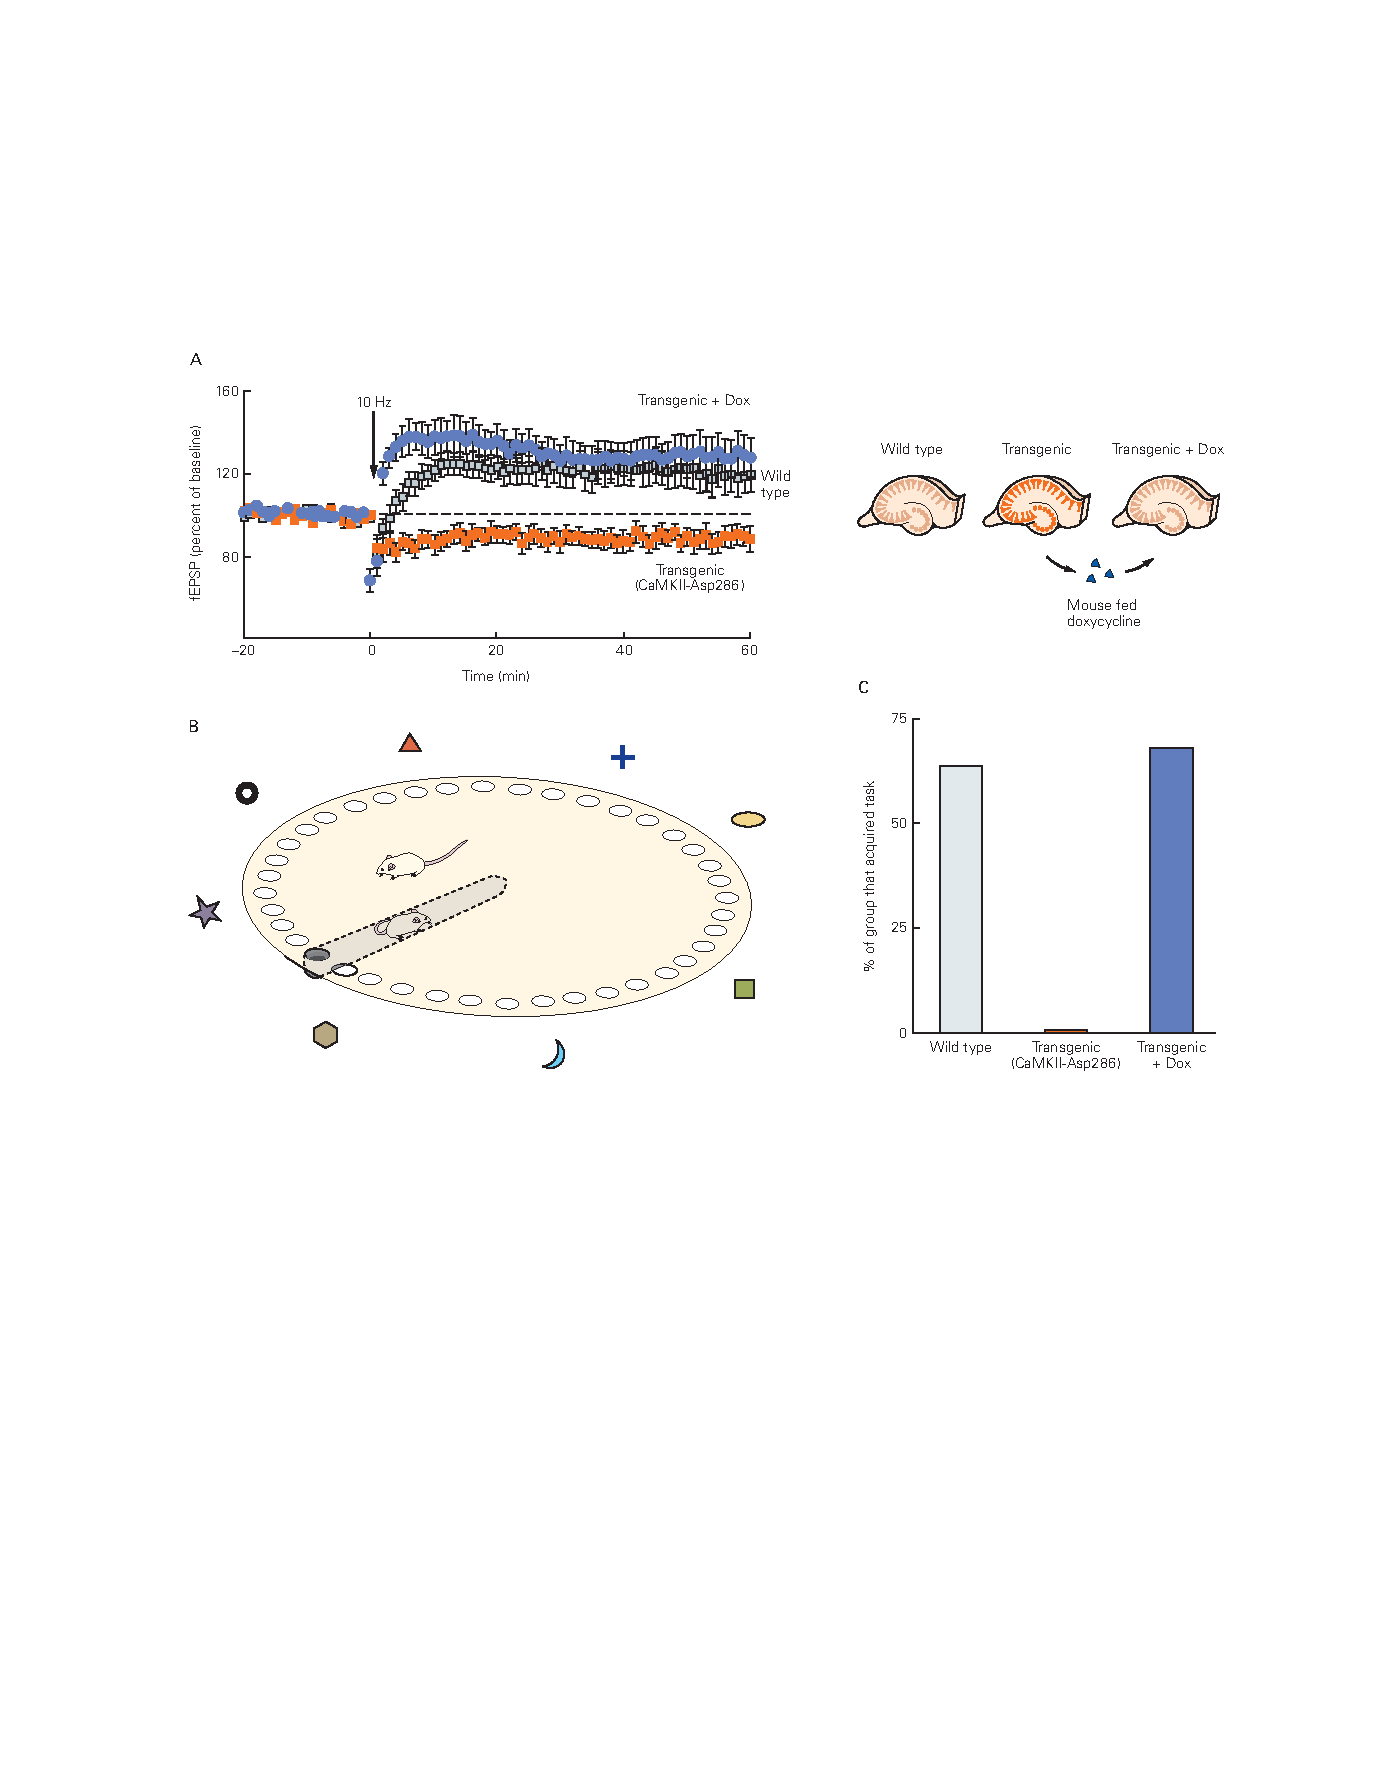
\includegraphics[width=0.9\linewidth]{chap54/fig_54_9}
	\caption{转基因引起的长时程增强 (LTP) 和空间记忆缺陷是可逆的。 (经许可转载自 Mayford 等人,1996 年。) A. 在来自过度表达 CaMKII-Asp286 激酶(CaMKII 的组成型活性突变体)的转基因小鼠的海马切片中观察到 LTP 缺陷。 该转基因的表达由第二个转基因驱动,即 tTA 细菌转录因子,它被抗生素多西环素 (Dox) 抑制(有关完整描述,请参见第 \ref{chap:chap2} 章图 2-9)。 测试了四组小鼠:喂食多西环素的转基因小鼠,多西环素可阻断激酶的表达; 不含多西环素的转基因小鼠,其中表达激酶; 和野生型小鼠有和没有多西环素。 在野生型小鼠中,10 赫兹的破伤风会诱发 LTP; 多西环素没有作用(数据未显示)。 在转基因小鼠中,破伤风不能诱导 LTP,但会引起小的突触抑制。 在喂食多西环素的转基因小鼠中,LTP 缺陷得到逆转。 (缩写:fEPSP,场兴奋性突触后电位。) B. 在 Barnes 迷宫中测试了激酶对空间记忆的影响。 迷宫由一个有 40 个孔的平台组成,其中一个孔通向允许老鼠离开平台的逃生隧道。 鼠标放置在平台的中央。 老鼠不喜欢开阔、光线充足的空间,因此试图通过找到通向逃生隧道的洞来逃离平台。 学习和记住孔位置的最有效方法(也是满足实验者为任务设定的标准的唯一方法)是老鼠使用四壁上的独特标记作为空间线索,从而展示海马空间 记忆。 C. 接受多西环素的转基因小鼠在学习巴恩斯迷宫任务方面表现与野生型小鼠一样好(大约 65\% 的动物学习该任务),而没有接受多西环素的转基因小鼠(因此表达 CaMKII-Asp286)不学习该任务 .}
	\label{fig:54_9}
\end{figure}


这些使用\textit{N-甲基-D-天冬氨酸}受体的限制性敲除和过表达以及 CaMKII-Asp286 的受控过表达的几个实验清楚地表明,空间记忆也需要对 Schaffer 侧支突触的 LTP 很重要的分子途径。
然而,这样的结果并没有直接表明空间学习和记忆实际上与海马突触传递的增强有关。
Mark Bear 和他的同事通过监测大鼠体内 Schaffer 侧支突触的突触传递强度解决了这个问题。


使用一系列细胞外电极刺激 Schaffer 侧支输入,并使用另一个阵列记录不同位置的细胞外场 EPSP,记录突触强度。
然后通过足部电击训练大鼠避开箱子的一侧;
训练后重新测量现场 EPSP,显示记录电极子集的突触传输幅度有小幅但显着的增加。
学习过程中突触传递的增加是由 LTP 还是其他机制引起的?
因为给定突触的 LTP 数量是有限的,如果学习确实招募了类似 LTP 的过程,那么学习后强直刺激诱导 LTP 的能力应该会降低。
事实上,Bear 和他的同事们发现,在那些行为训练在现场 EPSP 中产生最大增强的记录点,LTP 的量级减少了。
这一结果类似于杏仁核中的发现,其中恐惧学习降低了由随后的强直性刺激引起的 LTP 的强度。


如果类似 LTP 的变化发生在海马体的记忆形成过程中,那么这种变化只会发生在一小部分突触中,即那些参与特定记忆存储的突触。
不同的记忆可能对应于具有增强的突触互连的不同细胞集合。
然而,如果这是真的,那么海马体记忆应该很容易被不加区别地改变整个网络内突触强度的操作所破坏。
为了验证这个想法,研究人员在水迷宫任务中依赖海马体的空间训练后,在整个齿状回中诱导了 LTP。
该协议确实会损害动物对水迷宫中目标位置的记忆。
在学习之后但在高频刺激之前给予\textit{N-甲基-D-天冬氨酸}受体拮抗剂的对照动物表现出正常的空间记忆。
这些结果表明,记忆障碍是由于不分青红皂白的 LTP 的产生而产生的,这可能会破坏编码目标位置记忆的强突触和弱突触的特定模式。


最后,尽管 LTP 的大多数行为测试都使用空间学习任务来评估记忆,但研究还表明,\textit{N-甲基-D-天冬氨酸}受体以及推断的 LTP 对各种依赖于海马体的外显记忆是必需的。
当 CA1 区域的\textit{N-甲基-D-天冬氨酸}受体被阻断时,小鼠无法掌握非空间物体识别任务,学习复杂的气味辨别,或经历食物偏好的社会传播,其中动物通过观察食物来学习接受新食物 同种动物(同类的另一种动物)食用相同的食物。
因此,\textit{N-甲基-D-天冬氨酸}受体依赖性 LTP 可能是海马体中许多(如果不是全部)外显记忆形式所必需的(其中大部分包括空间识别元素)。



\section{显式记忆存储也依赖于突触传递的长期抑制}

如果突触连接只能增强而永远不会减弱,那么突触传递可能会迅速饱和——突触连接的强度可能会达到一个点,超过这个点就不可能进一步增强。
此外,统一的突触强化可能会导致记忆特异性丧失,一种记忆会干扰另一种记忆。
然而,个人能够在一生中学习、存储和回忆新的记忆。
这个悖论导致了这样的建议,即神经元必须具有下调突触功能以抵消 LTP 的机制。


这种被称为长期抑郁症 (LTD) 的抑制机制最初是在小脑中发现的,它对运动学习很重要。
从那时起,LTD 也在海马体中的许多突触中得到表征。 LTP 通常是由短暂的高频破伤风引起的,而 LTD 是由长时间的低频突触刺激引起的(图 \ref{fig:54_10}A)。
如上所述,它也可以通过尖峰配对协议诱导,其中 EPSP 在突触后细胞中的动作电位后被诱发。
这暗示了 Hebb 学习规则的一个推论:对细胞放电没有贡献的活跃突触被削弱。
与 LTP 一样,在 LTD 的诱导和表达过程中涉及许多分子和突触机制。


\begin{figure}[htbp]
	\centering
	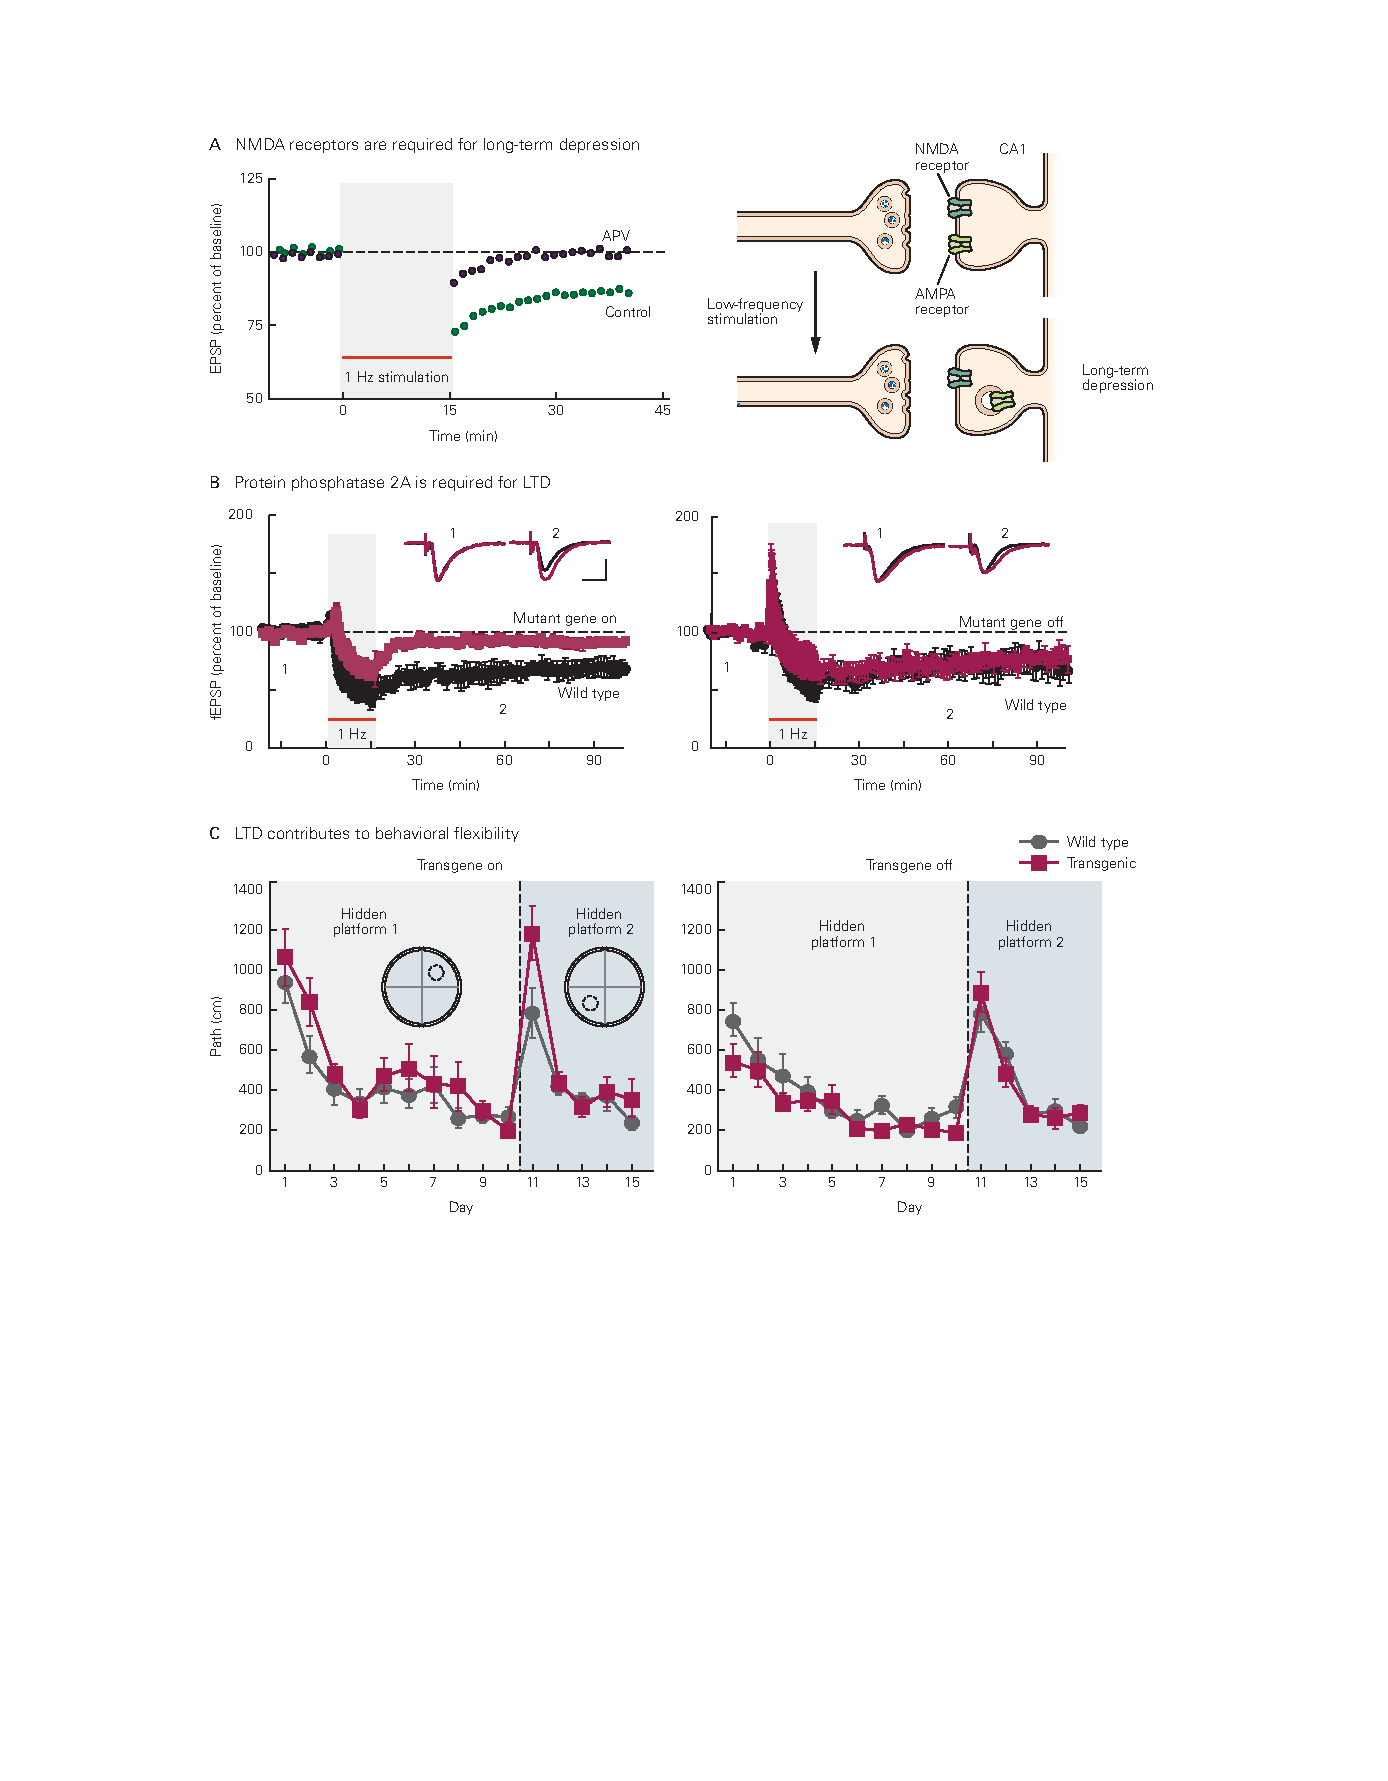
\includegraphics[width=0.95\linewidth]{chap54/fig_54_10}
	\caption{突触传递的长期抑制需要\textit{N-甲基-D-天冬氨酸}受体和磷酸酶活性。 A. 对 Schaffer 侧支纤维的长时间低频刺激(1 Hz,15 分钟)会导致海马 CA1 区场兴奋性突触后电位 (fEPSP) 的大小长期下降,这种下降比刺激持续时间更长 (控制)。 当 α-amino-3-hydroxy-5-methyl-4-isoxazolepropionic acid (AMPA) 受体通过内吞作用从突触后膜移除时,会发生长期抑郁症 (LTD); 当 NMDA 受体被药物 2-amino-5-phosphonovaleric acid (APV) 阻断时,它被阻断。 (改编自 Dudek 和 Bear 1992。)B. LTD 需要蛋白质去磷酸化。 该图比较了野生型小鼠和表达抑制磷蛋白磷酸酶 2A 的蛋白质的转基因小鼠海马 CA1 区的 LTD。 转基因表达受 tTA 系统控制。 在没有多西环素的情况下,表达磷酸酶抑制剂,并抑制 LTD 的诱导(左图)。 当通过施用多西环素关闭磷酸酶抑制剂的表达时,会诱导正常大小的 LTD(右图)。 C. 抑制磷酸酶 2A 会降低行为灵活性。 表达磷酸酶抑制剂的转基因小鼠以与野生型小鼠相同的速度(第 1-10 天)学习莫里斯迷宫中水下平台的位置。 因此,LTD 不是学习初始平台位置所必需的。 在第 10 天结束时,平台被移动到一个新的隐藏位置并重新测试小鼠(第 11-15 天)。 现在,转基因小鼠在重新测试的第一天(第 11 天)要走更长的路才能找到平台,这表明学习受损(灵活性降低)。 当用多西环素关闭转基因表达时,转基因小鼠在测试的所有阶段都表现出正常的学习能力。 (面板 B 和 C 经许可转载自 Nicholls 等人,2008 年。)}
	\label{fig:54_10}
\end{figure}


令人惊讶的是,许多形式的 LTD 需要激活 LTP 中涉及的相同受体,即\textit{N-甲基-D-天冬氨酸}受体(图~\ref{fig:54_10}A)。
单一类型受体的激活如何同时产生增强和抑制?
一个关键的区别在于用于诱导 LTP 或 LTD 的实验方案。
与用于诱导 LTP 的高频刺激相比,用于诱导 LTD 的低频破伤风产生相对适度的突触后去极化,因此在缓解\textit{N-甲基-D-天冬氨酸}受体的 Mg2+ 阻滞方面效果要差得多。
因此,突触后细胞中 Ca2+ 浓度的任何增加都比 LTP 诱导期间观察到的增加小得多,因此不足以激活 CaMKII,LTP 中涉及的酶。
相反,LTD 可能是由钙依赖性磷酸酶钙调神经磷酸酶的激活引起的,钙调神经磷酸酶是一种酶复合物,与 CaMKII 相比,它对 Ca2+ 具有更高的亲和力(第 \ref{chap:chap14} 章)。


长期抑郁症也可能取决于离子型\textit{N-甲基-D-天冬氨酸}受体通道令人惊讶的促代谢作用。
除了打开受体孔之外,谷氨酸结合被认为会引发受体胞质结构域的构象变化,从而直接激活下游信号级联反应,从而增加磷蛋白磷酸酶 1 (PP1) 的活性。
PP1 或钙调神经磷酸酶的激活最终导致蛋白质磷酸化的变化,从而促进 AMPA 受体的内吞作用,从而导致 EPSP 大小的减小。


通过激活 G 蛋白偶联的代谢型谷氨酸受体,可以诱导截然不同的 LTD 形式。
这种形式的 LTD 取决于有丝分裂原活化蛋白 (MAP) 激酶信号通路的激活(第 \ref{chap:chap14} 章),而不是磷酸酶的激活。
这些类型的 LTD 通过减少从突触前末端释放的谷氨酸以及通过改变突触后细胞中 AMPA 受体的运输来导致突触传递减少。


与 LTP 相比,LTD 的行为作用知之甚少,但一些见解来自使用表达蛋白磷酸酶抑制剂的转基因小鼠的研究。
依赖于\textit{N-甲基-D-天冬氨酸}受体的 LTD 在转基因表达时受到抑制,但在转基因表达受到抑制时正常(图~\ref{fig:54_10}B)。
转基因表达不影响 LTP 或涉及代谢型谷氨酸受体的 LTD 形式。
表达转基因的小鼠在 Morris 迷宫中第一次测试时表现出正常的学习能力。
然而,当隐藏平台移动到新位置后再次测试相同的老鼠时,它们学习新位置的能力下降,并且倾向于坚持搜索靠近先前学习位置的平台(图 \ref{fig:54_10}C)。
因此,LTD 可能不仅是防止 LTP 饱和所必需的,而且对于增强记忆存储的灵活性和记忆召回的特异性也是必需的。
对恐惧条件反射的研究表明,杏仁核中的 LTD 可能对逆转习得性恐惧很重要。



\subsection{记忆存储在单元组件中}

虽然长期突触可塑性和记忆形成之间关系的累积证据很强,但我们对 LTP 等特定细胞过程如何促进记忆形成知之甚少。
这反映了我们对神经回路如何运作以及记忆如何嵌入其中的知识的局限性。
神经回路中记忆存储的理论模型可以追溯到 Hebb 的细胞集合概念——每当执行功能时就会激活的神经元网络;
例如,每次回忆时。
一个集合中的细胞通过在记忆形成时加强的兴奋性突触连接结合在一起。


半个多世纪后的今天,尽管很难获得实验证据,但赫布的思想仍然构成了海马体如何调节记忆的存储和回忆的框架。
适当的测试需要同时记录数千个神经元的活动,并结合选定细胞群的实验性激发或失活。
技术进步现在使此类实验成为可能。
总的来说,到目前为止获得的结果证实了 Hebb 的细胞组装模型,并暗示 LTP 是它们形成的机制。


在对小鼠进行的一项有意义的研究中,Susumu Tonegawa 和他的同事测试了参与特定记忆存储的神经元的重新激活是否足以触发该记忆的回忆。
研究人员首先对探索新环境的动物进行电击。
一天或更长时间后将动物再次暴露于相同环境会引起冻结反应,表明动物将环境或环境(条件刺激)与电击(非条件刺激)相关联。
使用遗传策略,Tonegawa 导致在恐惧条件反射期间活跃的齿状回颗粒神经元子集表达光激活阳离子通道 channelrhodopsin-2(图 \ref{fig:54_11})。
随后将条件动物置于与条件环境不同的新环境中,因此不会引起恐惧反应。
然而,即使动物处于非威胁性环境中,在恐惧条件反射期间活跃的颗粒细胞亚群的光激活也能够引发强烈的冻结反应。
这支持了记忆存储在细胞集合中的观点,更重要的是,证明了这些集合的重新激活足以引发对经历的回忆。


\begin{figure}[htbp]
	\centering
	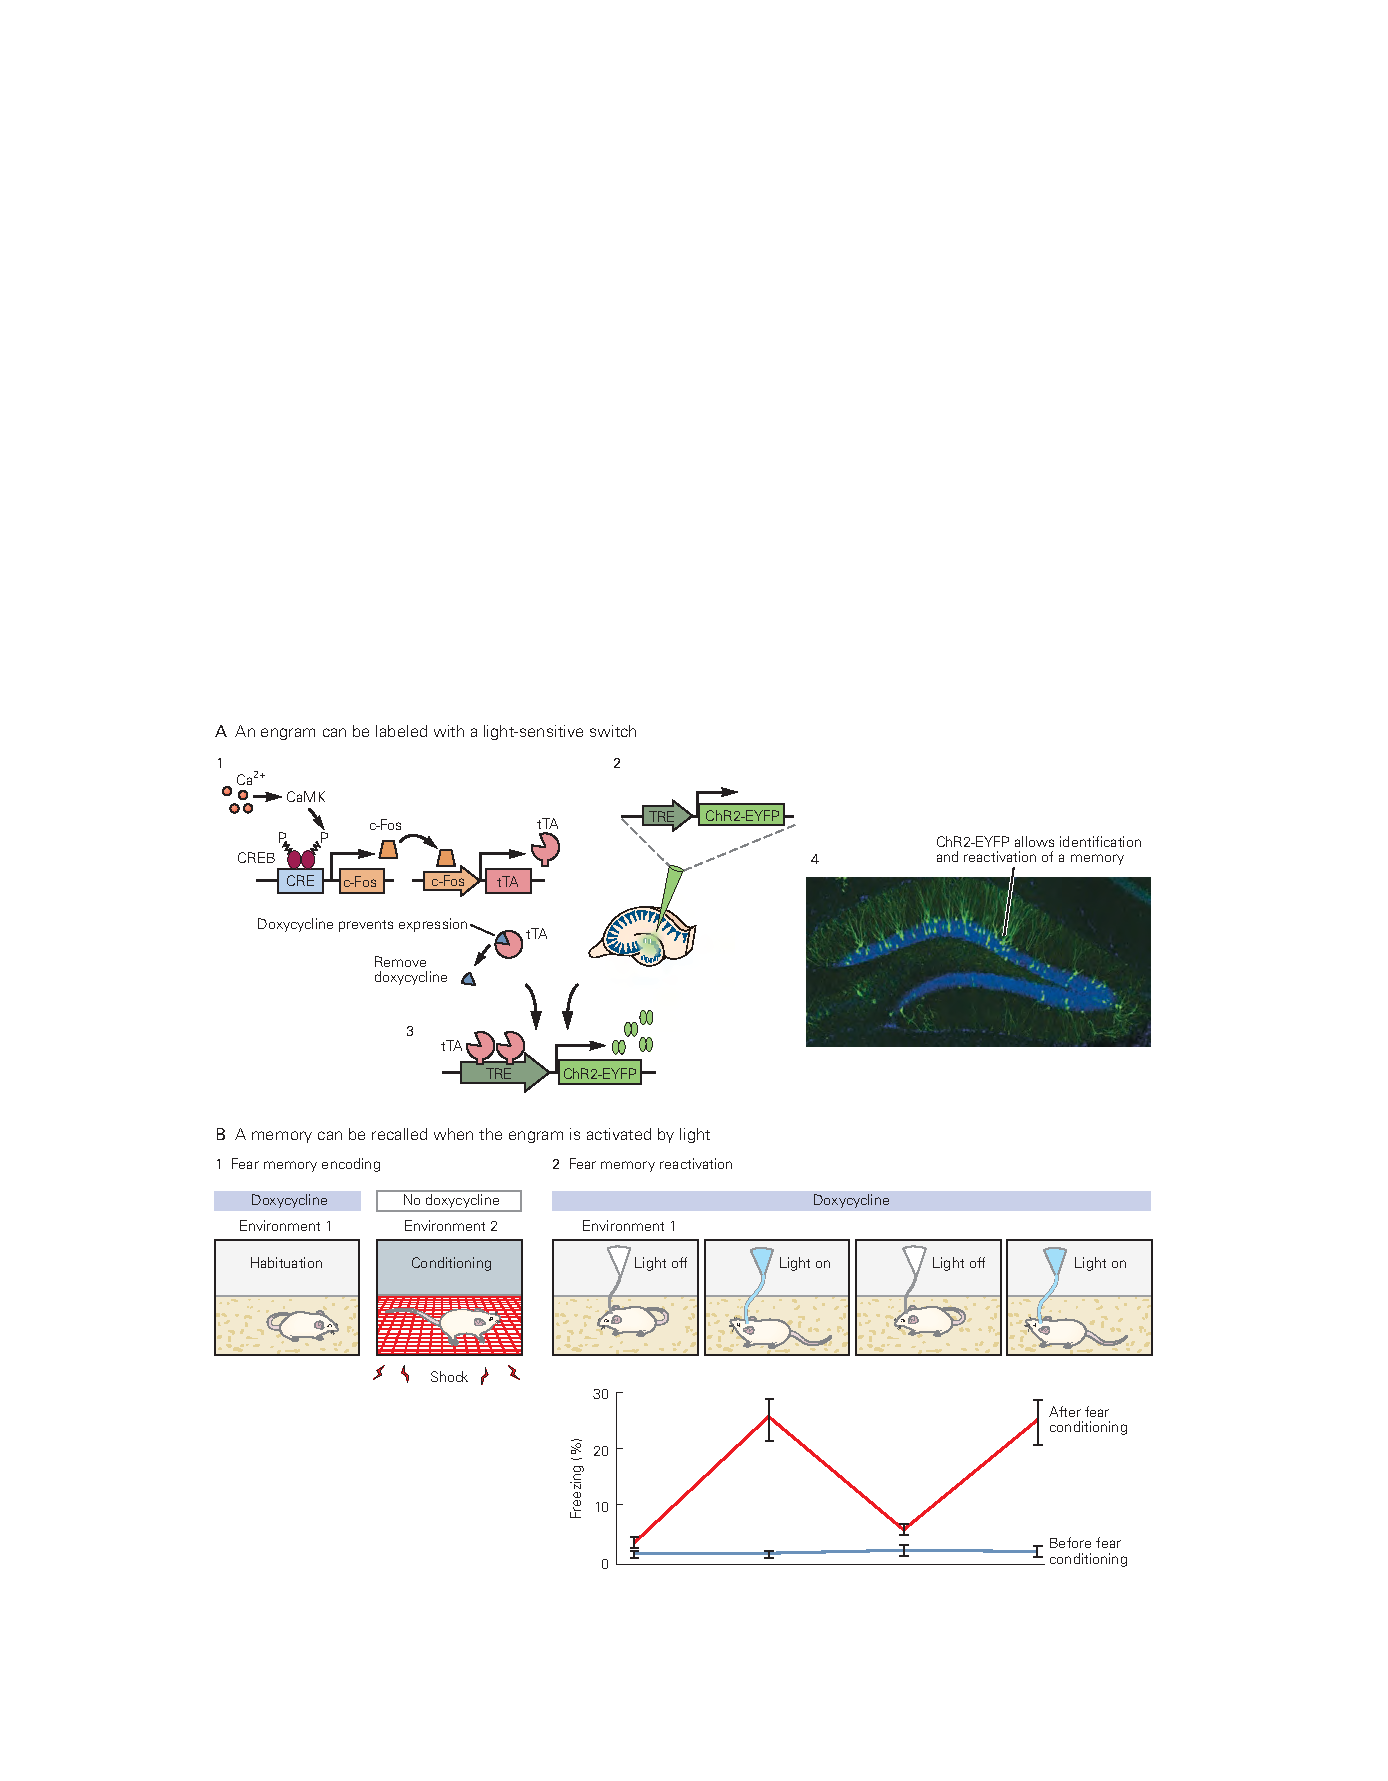
\includegraphics[width=0.9\linewidth]{chap54/fig_54_11}
	\caption{刺激与存储的恐惧调节记忆相关的神经元集合会引发恐惧行为。 (经 Liu et al. 2012 许可,面板复制或重新绘制。版权所有 © 2012 Springer Nature。)A. 实验方案。 1. 将小鼠暴露于新环境会增加一组为环境编码的海马神经元(细胞集合)的活动。 该活性增加细胞内 Ca2+,从而激活 CaM 激酶信号级联,导致转录因子 CREB 磷酸化。 磷酸化的 CREB 会增加即刻早期基因的表达,包括 c-Fos 转录因子。 在 c-fos-tTA 转基因小鼠系中,c-Fos 与转基因的 c-fos 启动子结合,从而启动转录因子 tTA 的表达。 将抗生素多西环素喂给小鼠,它会结合并抑制 tTA,直到实验当天。 2. 相同转基因小鼠的齿状回预先注射了一种腺相关病毒,该病毒含有编码 ChR2 的\textit{脱氧核糖核酸}序列,该序列与荧光标记蛋白 EYFP (ChR2-EYFP) 融合。 该序列的转录在 TRE 启动子的控制下,需要 tTA(不含多西环素)进行表达。 3. 将小鼠暴露于新环境(从饲料中去除多西环素后)会导致 tTA 的表达以及随后在活跃的齿状回神经元子集中表达 ChR2-EYFP。 4. ChR2-EYFP 在神经元中保持表达数天,如海马切片中齿状回颗粒细胞中的 EYFP 荧光信号所见。 (ChR2-EYPF 为绿色,齿状回细胞体层为蓝色。) B. 恐惧记忆的回忆。 在齿状回上方植入光纤。 1. 在恐惧记忆编码过程中,小鼠首先在一个环境中适应,同时喂食多西环素(可防止 ChR2-EYFP 的表达)。 然后将小鼠从多西环素中取出并暴露在新环境中几分钟。 这开启了在新环境中活跃的神经元集合中的基因转录,导致这些细胞中 ChR2-EYFP 的表达延长。 然后在新环境中对小鼠进行一系列电击以诱发恐惧条件反射:小鼠学会将新环境与恐惧刺激相关联。 然后将小鼠放回笼子并重新服用多西环素。 2. 在调节后 5 天的恐惧记忆重新激活期间,小鼠在重新进入接受电击的环境(未显示)时表现出正常的防御性冻结行为。 然而,当小鼠暴露于它们最初习惯的环境(没有相关的足部电击)时,它们通常将此识别为中性环境并且不会表现出防御性冻结。 然而,当小鼠探索中性环境时,传递蓝光以激活齿状回中表达 ChR2 的神经元会导致小鼠冻结。 这表明最初在调节环境中激活的表达 ChR2 的神经元群的激活足以唤起与该环境相关的恐惧记忆。 实验数据表明,与关灯时相比,打开光脉冲时,中性环境中的冻结响应要大得多(红色图;顶部卡通中指示的光传输)。 将光脉冲传递给没有经历过恐惧条件反射的动物不会引起冻结(蓝色图)。}
	\label{fig:54_11}
\end{figure}


在补充实验方法中,光激活抑制性 Cl- 转运蛋白在恐惧调节时活跃的 CA1 细胞中表达。
后来,标记的细胞被灭活,动物再次被置于它们受到电击的环境中。
在这些条件下,正常的冻结行为(即回忆恐惧条件反射的记忆)被阻断,表明标记的 CA1 细胞群中的活动对于记忆检索是必需的。
综上所述,这些发现表明,编码期间发生的特定细胞组装模式的重新激活对于记忆检索既是必要的也是充分的。


也许对集成模型最直接的测试是错误记忆的创建。 Tonegawa 及其同事在探索新环境(背景 A)期间活跃的细胞中表达通道视紫红质,只是这次没有发出电击。
稍后,当小鼠探索第二个新环境(环境 B)时,使用光刺激重新激活标记的细胞,这次结合电击。
当这些动物回到中性情境 A 时,它们僵住了,尽管它们从未在这种环境中受到过电击。
这一结果表明,当与情境 B 中的厌恶经历配对时,情境 A 的原始印迹的重新激活能够产生错误记忆,导致动物害怕情境 A。
因此,可以修改 a 的行为意义 通过将装配与与原始体验无关的新体验配对,神经表征(响应给定刺激的神经放电模式)。



\section{海马体的不同分区处理外显记忆的不同方面}

外显记忆存储事实(语义记忆)、地点(空间记忆)、其他个体(社会记忆)和事件(情景记忆)的知识。
如上所述,外显记忆的成功存储和回忆需要在局部细胞集内形成活动模式以避免记忆之间的混淆。
同时,海马体依赖记忆的一个重要心理特征是,通常一些线索就足以引发复杂记忆的回忆。
海马体如何执行所有这些不同的功能?
它的子区域是否具有专门的作用,或者记忆是海马体的单一功能?
至少在某些情况下,可以将关键功能分配给海马体的特定区域。



\subsection{齿状回对于模式分离很重要}

海马体如何存储不同的神经活动模式以响应需要记住的每一次经历,包括区分两个密切相关环境的模式?
关于神经回路如何完成这项任务(通常称为模式分离)的当代想法可以追溯到 David Marr 在 20 世纪 60 年代末和 70 年代初的理论工作。
在一篇关于小脑的具有里程碑意义的论文中,Marr 提出,苔藓纤维输入到大量小脑颗粒细胞上的广泛差异可能允许在该系统中进行模式分离。


这种“扩展重新编码”的想法,即通过将有限数量的输入投射到更大数量的突触目标细胞上,形成不同的放电模式,后来被其他人应用于海马体。
他们提出,海马模式分离是由于内嗅输入到齿状回中大量颗粒细胞上的分歧所致。 随后的实验研究结果大致符合这些理论建议:
在不同环境中记录的神经活动模式在齿状回和 CA3 中的差异比在内嗅皮质上游的一个突触中的差异更大。
齿状回也与模式分离有关,因为针对该区域的损伤或基因操作会损害大鼠和小鼠区分相似位置和环境的能力。


齿状回是神经科学中最出人意料的发现之一,新神经元的诞生或神经发生并不局限于发育的早期阶段。
在整个成年期,新的神经元不断从前体干细胞中诞生,并融入神经回路。
然而,成人神经发生仅限于两个大脑区域的颗粒神经元:嗅球中的抑制性颗粒细胞和齿状回的兴奋性颗粒神经元。 最近的实验结果提出了这样一种可能性,即成人中新生的颗粒神经元对于模式分离特别重要,即使它们只占颗粒细胞总数的一小部分。
刺激神经发生的程序增强了小鼠区分密切相关环境的能力。
除了那些在成人中新生的齿状回颗粒神经元之外的所有齿状回颗粒神经元的实验沉默似乎并不损害模式分离,这意味着它是新生神经元对模式分离最重要的。
尽管神经发生在模式分离和记忆编码中的作用仍存在一些不确定性,但目前正在探索增强神经发生的方法作为治疗不同类型与年龄相关的记忆丧失的手段。



\subsection{CA3 区域对于模式完成很重要}

外显记忆的一个关键特征是一些线索通常足以检索复杂的存储记忆。
Marr 在 1971 年的第二篇具有里程碑意义的论文中提出,CA3 锥体细胞的反复兴奋性连接可能是这一现象的基础。
他提出,当记忆被编码时,神经元活动模式被存储为活跃的 CA3 细胞之间连接的变化。
在随后的记忆检索过程中,重新激活这个存储的细胞集合的一个子集将足以激活编码记忆的整个原始神经集合,因为集合的细胞之间存在很强的循环连接。
这种恢复称为模式完成。


LTP 对于 CA3 网络中模式完成的重要性在小鼠研究中可见,其中\textit{N-甲基-D-天冬氨酸}谷氨酸受体被选择性地从 CA3 神经元中删除。
这些小鼠在 CA3 神经元之间的复发性突触处经历了 LTP 的选择性丢失,而在苔藓纤维和 CA3 神经元之间的突触处或在 CA3 和 CA1 神经元之间的 Schaffer 侧支突触处,LTP 没有变化。
尽管存在这种缺陷,小鼠仍显示出正常的学习和记忆能力,可以使用一整套空间线索在水迷宫中寻找水下平台。
然而,当小鼠被要求寻找空间线索较少的平台时,它们的表现会受损,这表明 CA3 神经元之间反复出现的突触处的 LTP 对于模式完成很重要。



\subsection{CA2 区域编码社会记忆}

比较齿状回和 CA3 和 CA1 区域的神经元表征的研究表明,每个区域在海马记忆的存储和检索中都有独特的功能。
最近的证据表明,CA2 区域在社会记忆中起着至关重要的作用,社会记忆是个体识别和记住自己物种(同种)其他成员的能力。
CA2 的遗传沉默会破坏小鼠记住与其他小鼠相遇的能力,但不会损害其他形式的海马体依赖性记忆,包括物体和地点的记忆。


CA2 区域在海马区域中也是独一无二的,因为它具有非常高水平的激素催产素和加压素受体,这些激素是社会行为的重要调节剂。
选择性刺激 CA2 神经元的加压素输入可以大大延长社交记忆的持续时间。
社会记忆还依赖于海马体腹侧区域的 CA1 神经元,该区域与情绪行为相关,接收来自 CA2 的重要输入。



\section{海马体形成外部世界的空间地图}

海马神经元如何编码外部环境的特征以形成空间位置的记忆,使动物能够导航到记住的目标?
20 世纪 40 年代末,认知心理学家爱德华托尔曼提出,大脑中的某个地方一定存在对环境的表征。
他将这些神经表征称为认知地图。
人们认为它们不仅可以形成内部空间地图,还可以形成心理数据库,其中存储与动物在环境中的位置相关的信息,类似于照片的 GPS 坐标。


托尔曼没有机会确定认知地图是否真的存在于大脑中,但在 1971 年,约翰奥基夫和约翰多斯特罗夫斯基发现,当动物定位时,大鼠海马 CA1 和 CA3 区域的许多细胞会选择性地放电 在特定环境中的特定位置。
他们称这些细胞为“位置细胞”,并将细胞在环境中优先发射的空间位置称为“位置场”(图 \ref{fig:54_12}A、B)。
当动物进入一个新环境时,新的位置场会在几分钟内形成,并稳定数周至数月。


\begin{figure}[htbp]
	\centering
	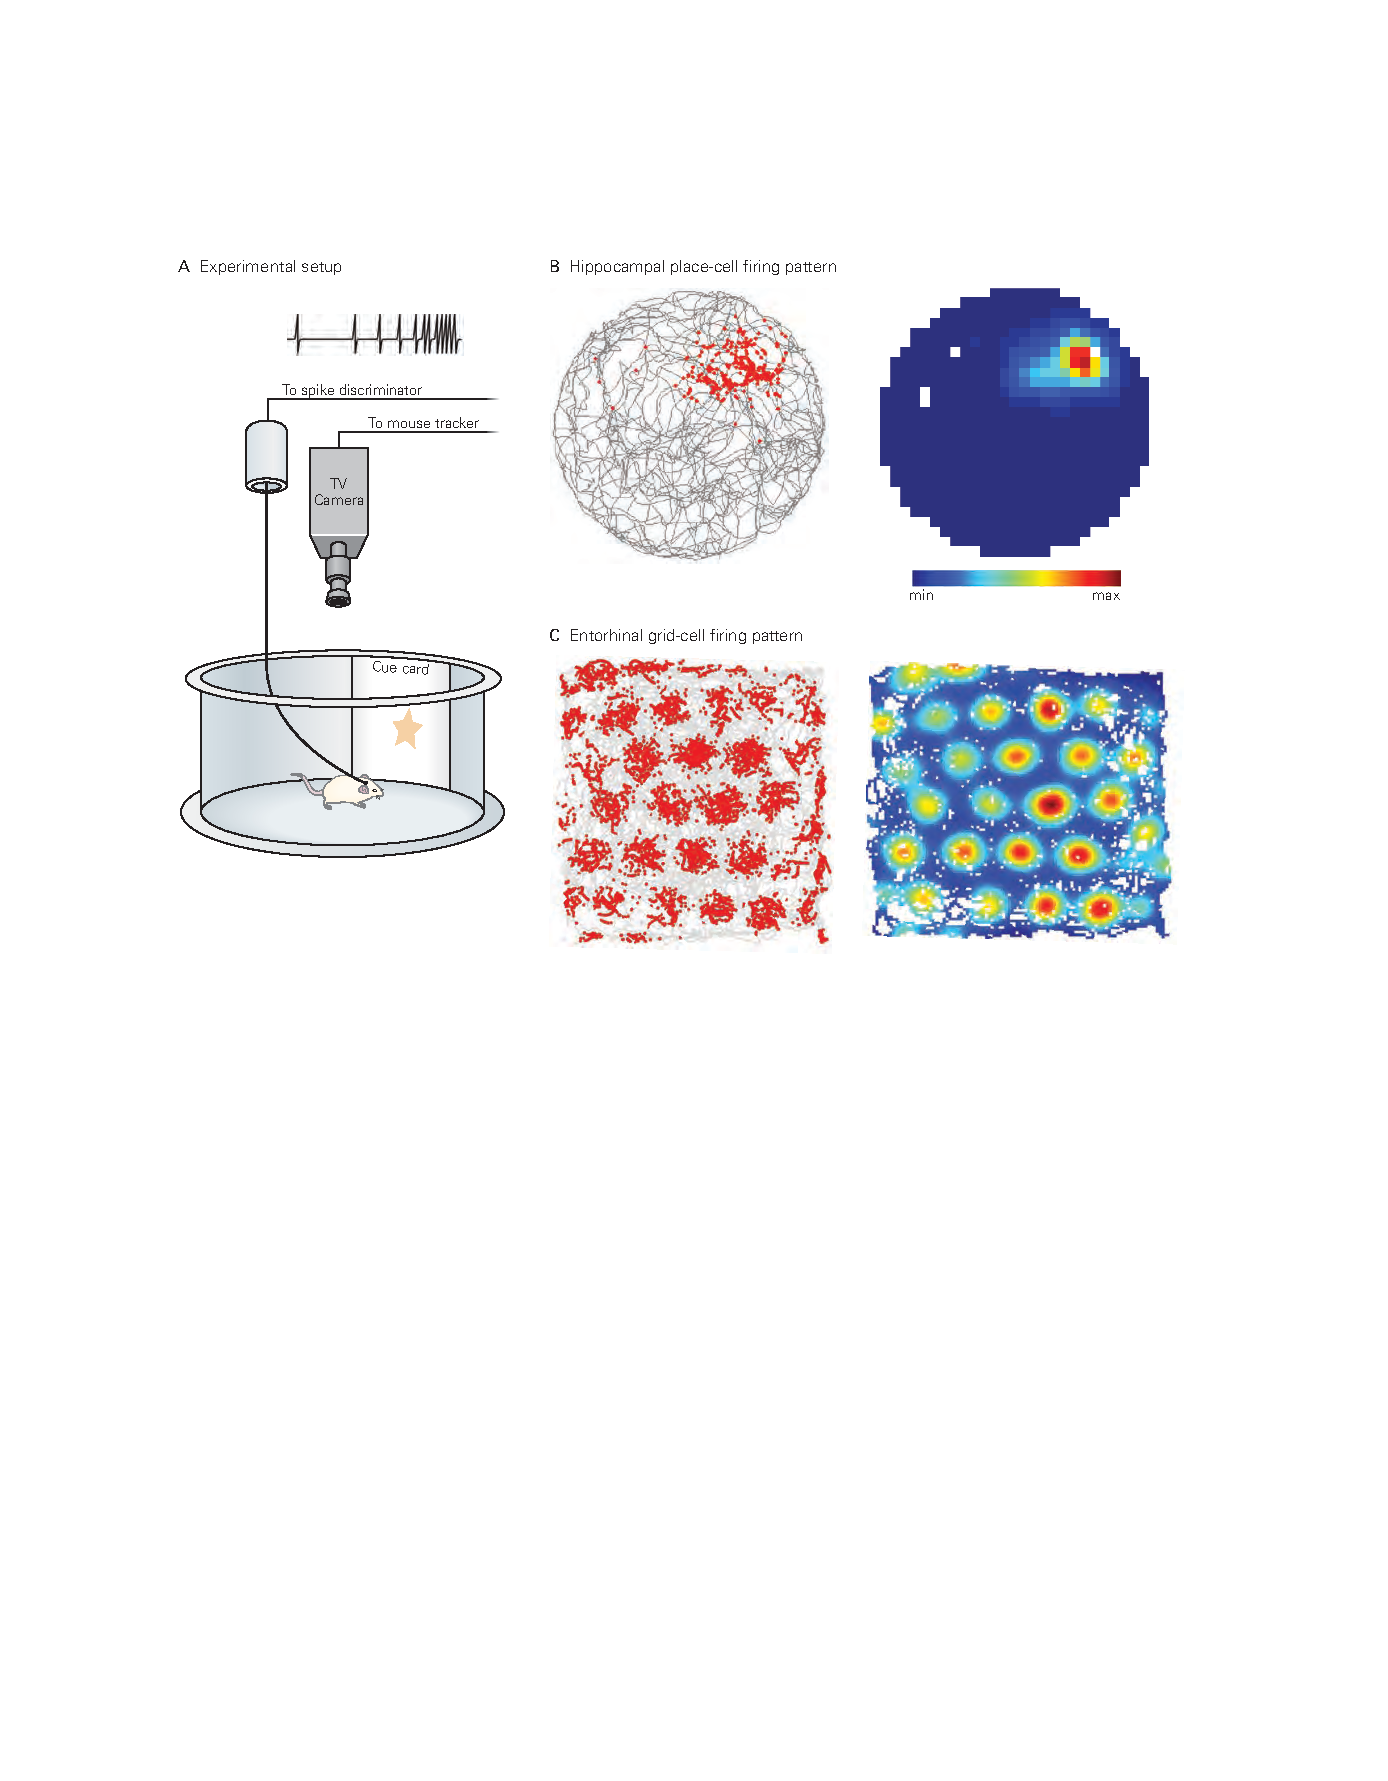
\includegraphics[width=0.9\linewidth]{chap54/fig_54_12}
	\caption{海马体和内侧内嗅皮质中细胞的放电模式表明动物在其周围环境中的位置。 A. 植入小鼠海马体的电极连接到记录电缆,该电缆连接到连接到基于计算机的尖峰识别程序的放大器。 鼠标被放置在带有高架电视摄像机的外壳中,该电视摄像机传输到检测鼠标位置的设备。 围栏还包含一个视觉提示来定位动物。 单个海马锥体神经元(“位置细胞”)中的尖峰由尖峰辨别程序检测。 然后绘制每个细胞的放电率作为动物在圆柱体中位置的函数。 此信息可视化为细胞的二维活动图,从中可以确定细胞的发射场(如 B 部分所示)。 (经许可改编自 Muller、Kubie 和 Ranck 1987。版权所有 © 1987 神经科学协会。) B. 海马体位置细胞的特定位置放电。 一只老鼠在类似于 A 部分所示的圆柱形围栏中奔跑。左图:围栏中动物的路径以灰色显示; 对于单个位置单元格,单个尖峰的发射位置显示为红点。 右图:同一细胞的放电率用颜色编码(蓝色 = 低率,红色 = 高率)。 在较大的环境中,位置细胞通常有一个以上的发射场,但这些场没有明显的空间关系。 C. 大鼠在 220 厘米宽的方形围栏中觅食 30 分钟期间内嗅网格细胞放电的空间模式。 该模式显示了典型的周期性网格发射场。 左:大鼠的轨迹以灰色显示; 个别峰值位置显示为红点。 右图:左侧网格单元的颜色编码发射率图。 B 部分中位置单元的颜色编码。(经许可改编自 Stensola 等人,2012 年。)}
	\label{fig:54_12}
\end{figure}


不同的位置细胞有不同的位置场,它们共同提供了一张环境地图,因为当前活跃的细胞的组合足以准确读出动物在环境中的位置。
位置细胞图在其组织中并不以自我为中心,就像大脑皮层表面的触觉或视觉神经图一样。
相反,它是非中心的(或地心的); 它相对于外部世界中的一个点是固定的。
基于这些特性,John O’Keefe 和 Lynn Nadel 在 1978 年提出,位置细胞是托尔曼心目中认知地图的一部分。
位置细胞的发现为环境的内部表征提供了第一个证据,这种内部表征允许动物有目的地在世界各地航行。



\subsection{内嗅皮层神经元提供独特的空间表征}

海马空间图是如何形成的?
从内嗅皮层到海马体位置细胞的传入连接携带什么类型的空间信息?
2005 年,关于内侧内嗅皮层中某些神经元形成的空间表征的惊人发现,其轴突提供了海马体穿孔通路输入的主要部分。
这些神经元以与海马体位置细胞非常不同的方式代表空间。
这些内嗅神经元(称为网格细胞)不会像位置细胞那样在动物处于独特位置时发射,而是在动物处于形成六边形网格状阵列的几个规则间隔位置中的任何一个时发射(图 \ref{fig:54_12}C)。
当动物在环境中移动时,不同的网格细胞被激活,这样整个网格细胞群的活动总是代表动物的当前位置。


网格允许动物在独立于上下文、地标或特定标记的类似笛卡尔的外部坐标系中定位自己。
网格细胞的放电模式在动物访问的所有环境中都有表现,包括在完全黑暗的环境中。
网格细胞激发与视觉输入的独立性意味着内在网络以及自我运动线索可以作为信息源,以确保在整个环境中系统地激活网格细胞。
由内嗅输入传递的网格化空间信息随后在海马体中转化为独特的空间位置,由位置细胞群的放电所代表,但这种转化如何发生仍有待确定。
自从 2005 年在大鼠的内侧内嗅皮质中发现网格细胞以来,它们已在小鼠、蝙蝠、猴子和人类中得到鉴定。
来自飞行蝙蝠的记录表明,网格细胞和位置细胞代表三维空间中的位置,表明皮质 - 海马空间导航系统的普遍性。
最后,有人提出灵长类动物的网格细胞可以编码多个感官坐标系中的位置,包括眼睛固定坐标。


网格细胞显示出它们的发射场和解剖组织之间的特征关系(图 \ref{fig:54_13})。
细胞网格场的 x、y 坐标(通常称为网格相位)在内侧内嗅皮层同一位置的细胞之间有所不同。
两个相邻单元格的 x,y 坐标通常与相隔较远的网格单元格的坐标不同。
相比之下,单个网格区域的大小和它们之间的间距通常从内侧内嗅皮层的背侧到腹侧在地形上增加,从背极的典型网格间距 30 到 40 厘米扩大到数米 一些位于腹极的细胞(图 \ref{fig:54_13}A)。
扩展不是线性的而是阶梯式的,表明网格单元网络是模块化的。


\begin{figure}[htbp]
	\centering
	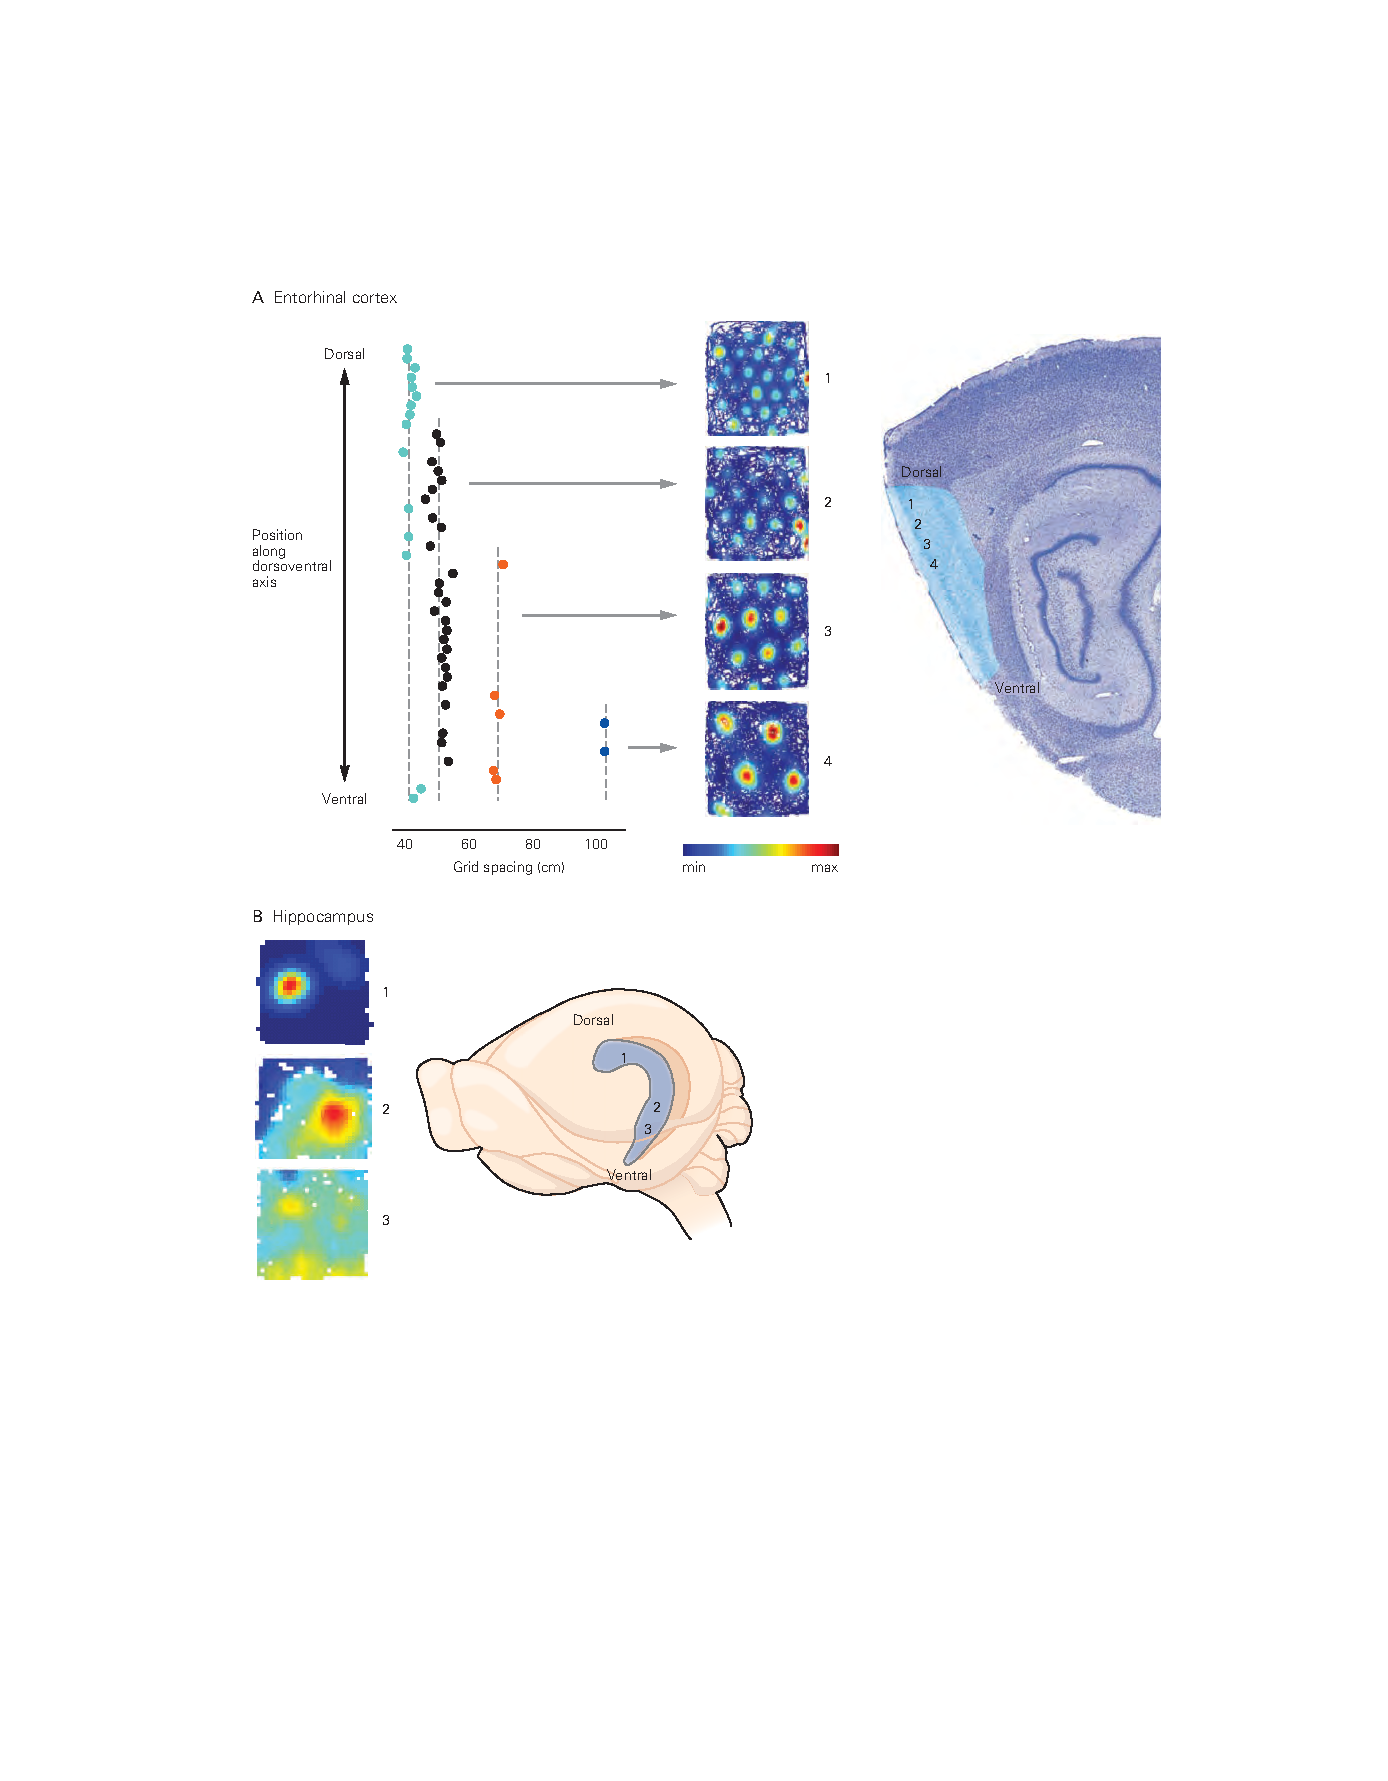
\includegraphics[width=0.8\linewidth]{chap54/fig_54_13}
	\caption{网格场和位置场的大小随着沿着内嗅皮层和海马体背腹轴的神经元位置而扩展。 A. 内嗅皮层网格尺度的地形组织。 网格间距(网格场之间的距离)是针对同一只大鼠在内侧内嗅皮质(右侧矢状脑部分的绿色区域)的连续背侧到腹侧水平记录的 49 个网格细胞(彩色点)确定的。 虚线表示平均网格间距值,表示网格间距落在四个离散模块之一中,点根据模块着色。 四个细胞的发射率图显示在中间(类似于图 54-12C)。 这些单元格的记录位置由右侧的数字 1 到 4 指示。 (经许可改编自 Stensola 等人,2012 年。)B. 沿海马背腹轴放置来自三个不同位置的场。 右图:海马结构中的记录位置(数字)如右图所示。 左图:颜色编码的地图显示记录位置处每个位置细胞的发射场。 视野大小在沿着海马背腹轴的细胞中扩展。 (经许可转载自 Kjelstrup 等人,2008 年。)}
	\label{fig:54_13}
\end{figure}


有趣的是,沿着海马体的背侧到腹侧轴,海马体位置细胞的位置区域的大小也逐渐扩大(图 \ref{fig:54_13}B)。
这与已知的突触连接模式一致:背侧内嗅皮质支配背侧海马体,而腹侧内嗅皮质支配腹侧海马体。
腹侧海马体位置场更大的发现与表明背侧海马体对空间记忆更重要的结果一致,而腹侧海马体对非空间记忆更重要,包括社会记忆和情绪行为。


网格细胞并不是唯一投射到海马体的内侧内嗅细胞。
其他包括头部方向细胞,它主要对动物所面对的方向作出反应(图 \ref{fig:54_14}A)。
这些细胞最初是在海马旁皮质的另一个区域前托下发现的,但它们也存在于内侧内嗅皮质中。
许多内嗅头部方向细胞也具有网格状的发射特性。
与网格细胞一样,当动物在二维环境中穿过三角形网格的顶点时,此类头部方向细胞会激活。
然而,在每个网格场内,这些细胞只有在动物面向特定方向时才会放电。
头部方向细胞和连接网格和头部方向细胞被认为为内嗅空间图提供方向信息。


\begin{figure}[htbp]
	\centering
	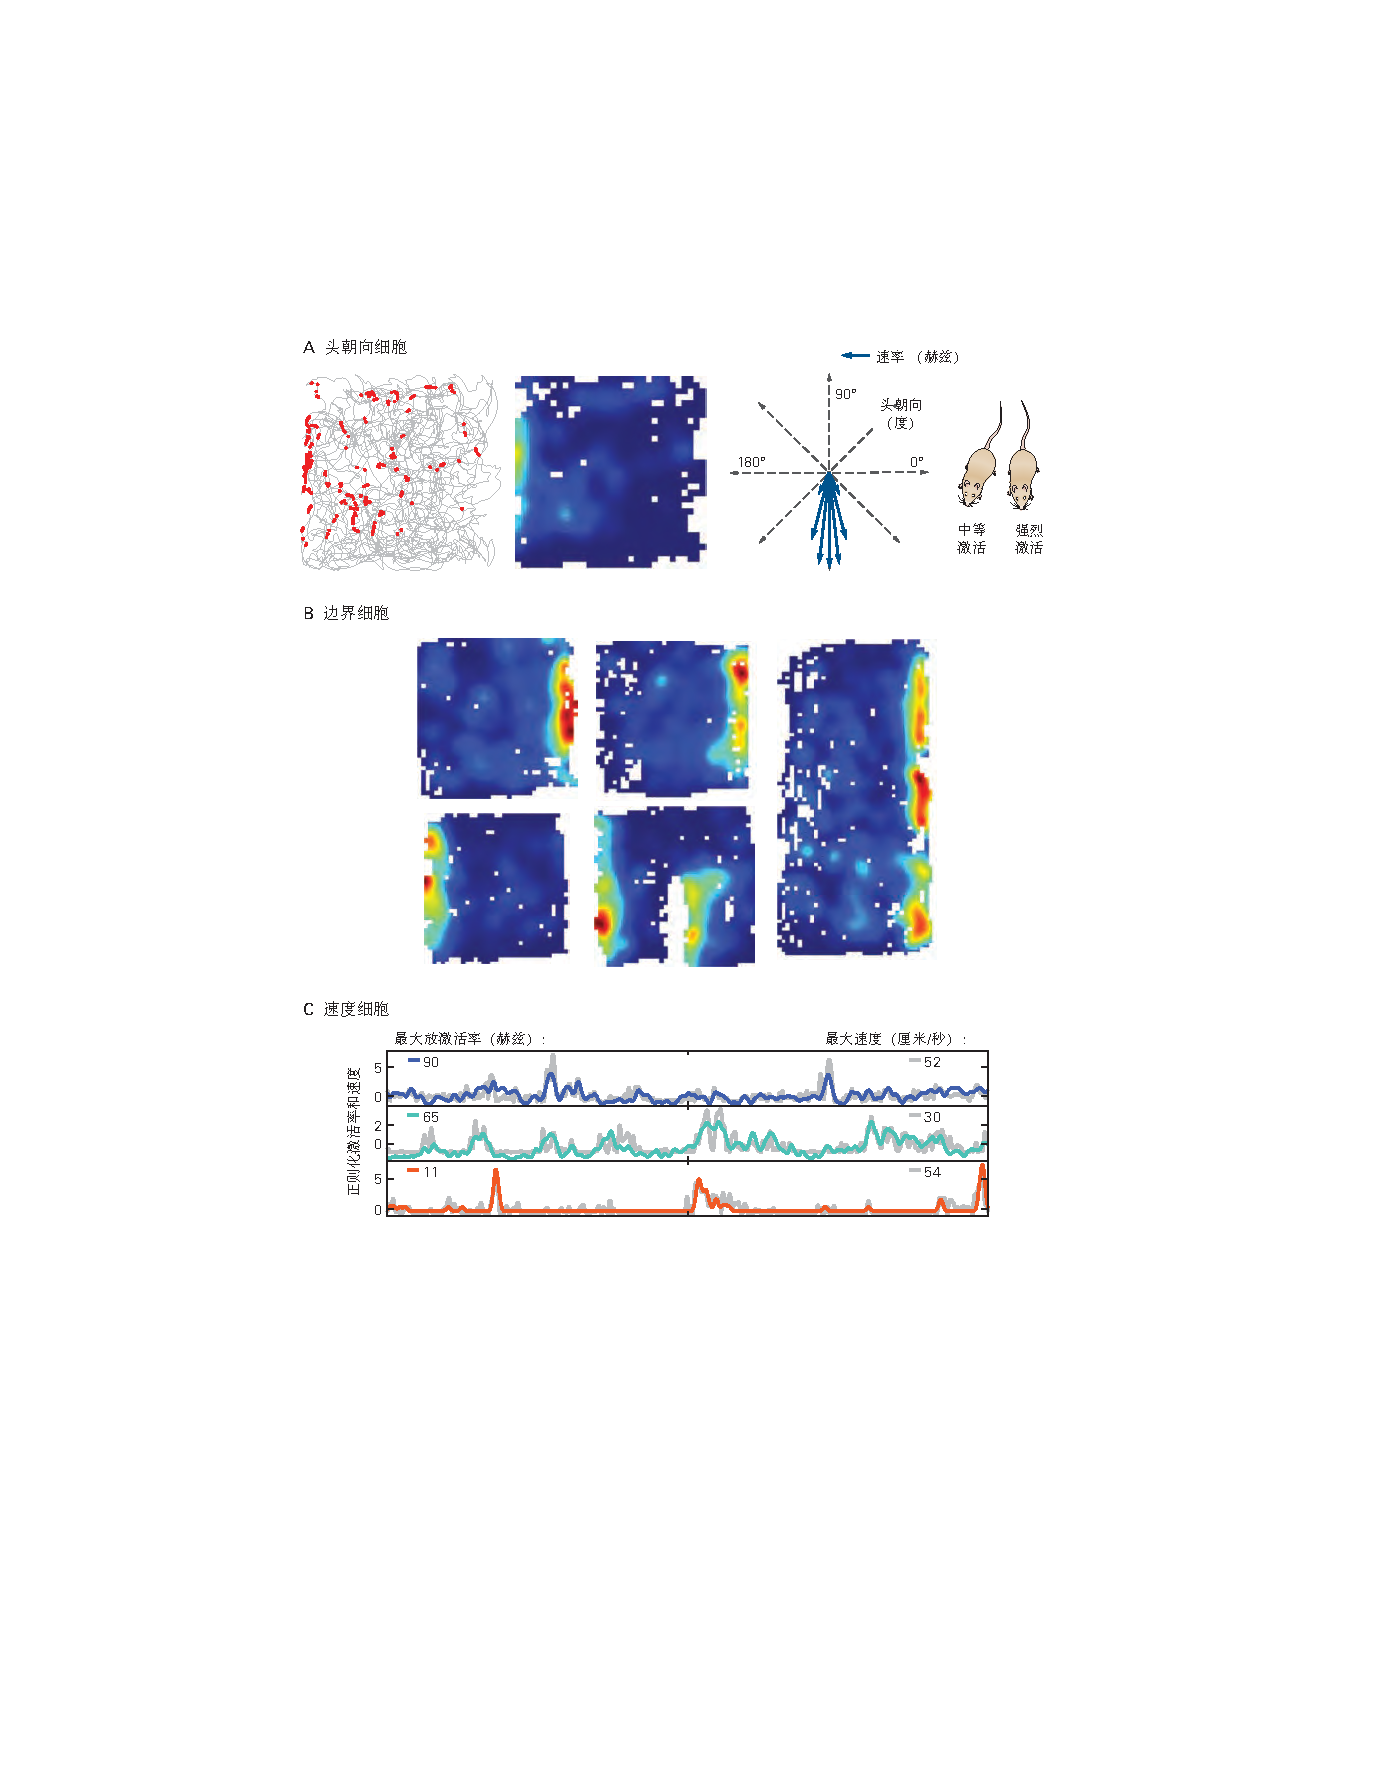
\includegraphics[width=0.7\linewidth]{chap54/fig_54_14}
	\caption{内侧内嗅皮层包含几种功能性细胞类型,可根据动物导航的不同表现进行调整。 A. 左边是一只老鼠在100厘米宽的方形围栏内探索的轨迹(红点表示开火位置)。 还显示了颜色编码的发射率图(颜色比例与之前的数字相同)。 请注意,电池的发射分散在整个外壳中。 右图以极坐标显示了同一细胞的放电率与头部方向的函数关系。 当老鼠面朝南方时,细胞会选择性地在盒子里的任何地方开火。 (经许可改编自 Sargolini 等人,2006 年。)B. 具有不同几何形状的外壳中具有代表性的边界单元的发射率图(红色 = 高速率;蓝色 = 低速率)。 顶行:当外壳从正方形(左图和中间图)拉伸为矩形(右图)时,射野图跟随墙壁。 底行:同一边界细胞在另一个环境中的射野。 在方形围栏内引入离散墙(白色像素,右图)会导致新的边界区域出现在墙的右侧。 (经许可转载自 Solstad 等人,2008 年。)C. 速度细胞。 迹线显示 2 分钟自由觅食期间七个代表性内嗅速度细胞的归一化发射率(彩色迹线)和速度(灰色)。 指示了射速和速度的最大值(分别为左和右)。 注意这些细胞中速度和发射率之间的高度对应。 (经许可转载自 Kropff 等人,2015 年。)}
	\label{fig:54_14}
\end{figure}


混合在网格单元和头部方向单元之间的是另一种类型的空间调制单元,即边界单元(图 \ref{fig:54_14}B)。
每当动物接近环境的局部边界(例如边缘或墙壁)时,边界细胞的放电率就会增加。
边界细胞可能有助于将网格细胞激发的相位和方向与环境的局部几何形状对齐。
最近发现的对象向量细胞可能扮演类似的角色——内侧内嗅皮质中的细胞编码动物相对于显着地标的距离和方向。
最后一种内嗅细胞类型是速度细胞。
速度细胞与动物的奔跑速度成正比,与动物的位置或方向无关(图 \ref{fig:54_14}C)。
与头部方向细胞一起,速度细胞可以为网格细胞提供有关动物瞬时速度的信息,从而允许活动网格细胞的集合根据移动动物的变化位置动态更新。


综上所述,这些发现指向内侧内嗅皮层中功能专用细胞网络,让人联想到感觉皮层的特征检测器。
每种细胞类型的功能特异性源于细胞对特定行为特征的表征。
从这个意义上说,内嗅细胞类型不同于大多数其他联合皮层中的细胞,后者以不易解码的方式整合来自许多来源的信息。


海马体和内侧内嗅皮质中的空间编码细胞之间的主要区别是什么?
所有内嗅细胞类型的一个显着特性是它们发射模式的刚性。
无论上下文或环境如何,共定位网格单元的集合都保持相同的内在激发模式。
当一对网格单元在一个环境中具有重叠的网格场时,它们的网格场在其他环境中也重叠。
如果它们的网格场是相反的,或者“异相”,它们在其他环境中也会是相反的。
在头部方向细胞和边界细胞中可以看到类似的刚性:
在一个环境中具有相似方向的细胞在其他环境中具有相似的方向。
速度单元还保持其对跨环境运行速度的独特调整。
这些发现表明,内侧内嗅皮层或该皮层回路的模块可能像一张无视环境细节的通用空间地图一样运作。
通过这样做,内嗅图与海马体的位置细胞图有很大不同。


海马体位置细胞的放电模式对环境变化非常敏感。
当动物的环境发生重大变化时,海马体中给定位置细胞的位置场通常会切换为编码完全不同的空间位置,这一过程称为“重新映射”。
有时,即使是感官或动机输入的微小变化也足以引发重新映射。
不同环境的海马体位置图缺乏相关性(图 \ref{fig:54_15})被认为有助于离散记忆的存储,并最大限度地降低一种记忆与另一种记忆混淆的风险,这一过程称为干扰。
对于像海马体这样的显性记忆系统来说,要存储数百万个事件,这可能是一个巨大的优势。
为了准确快速地表示动物在空间中的位置,如内侧内嗅皮层中发生的那样,使用对环境背景或非空间感官刺激不太敏感的更刻板的代码可能反而是有益的。


\begin{figure}[htbp]
	\centering
	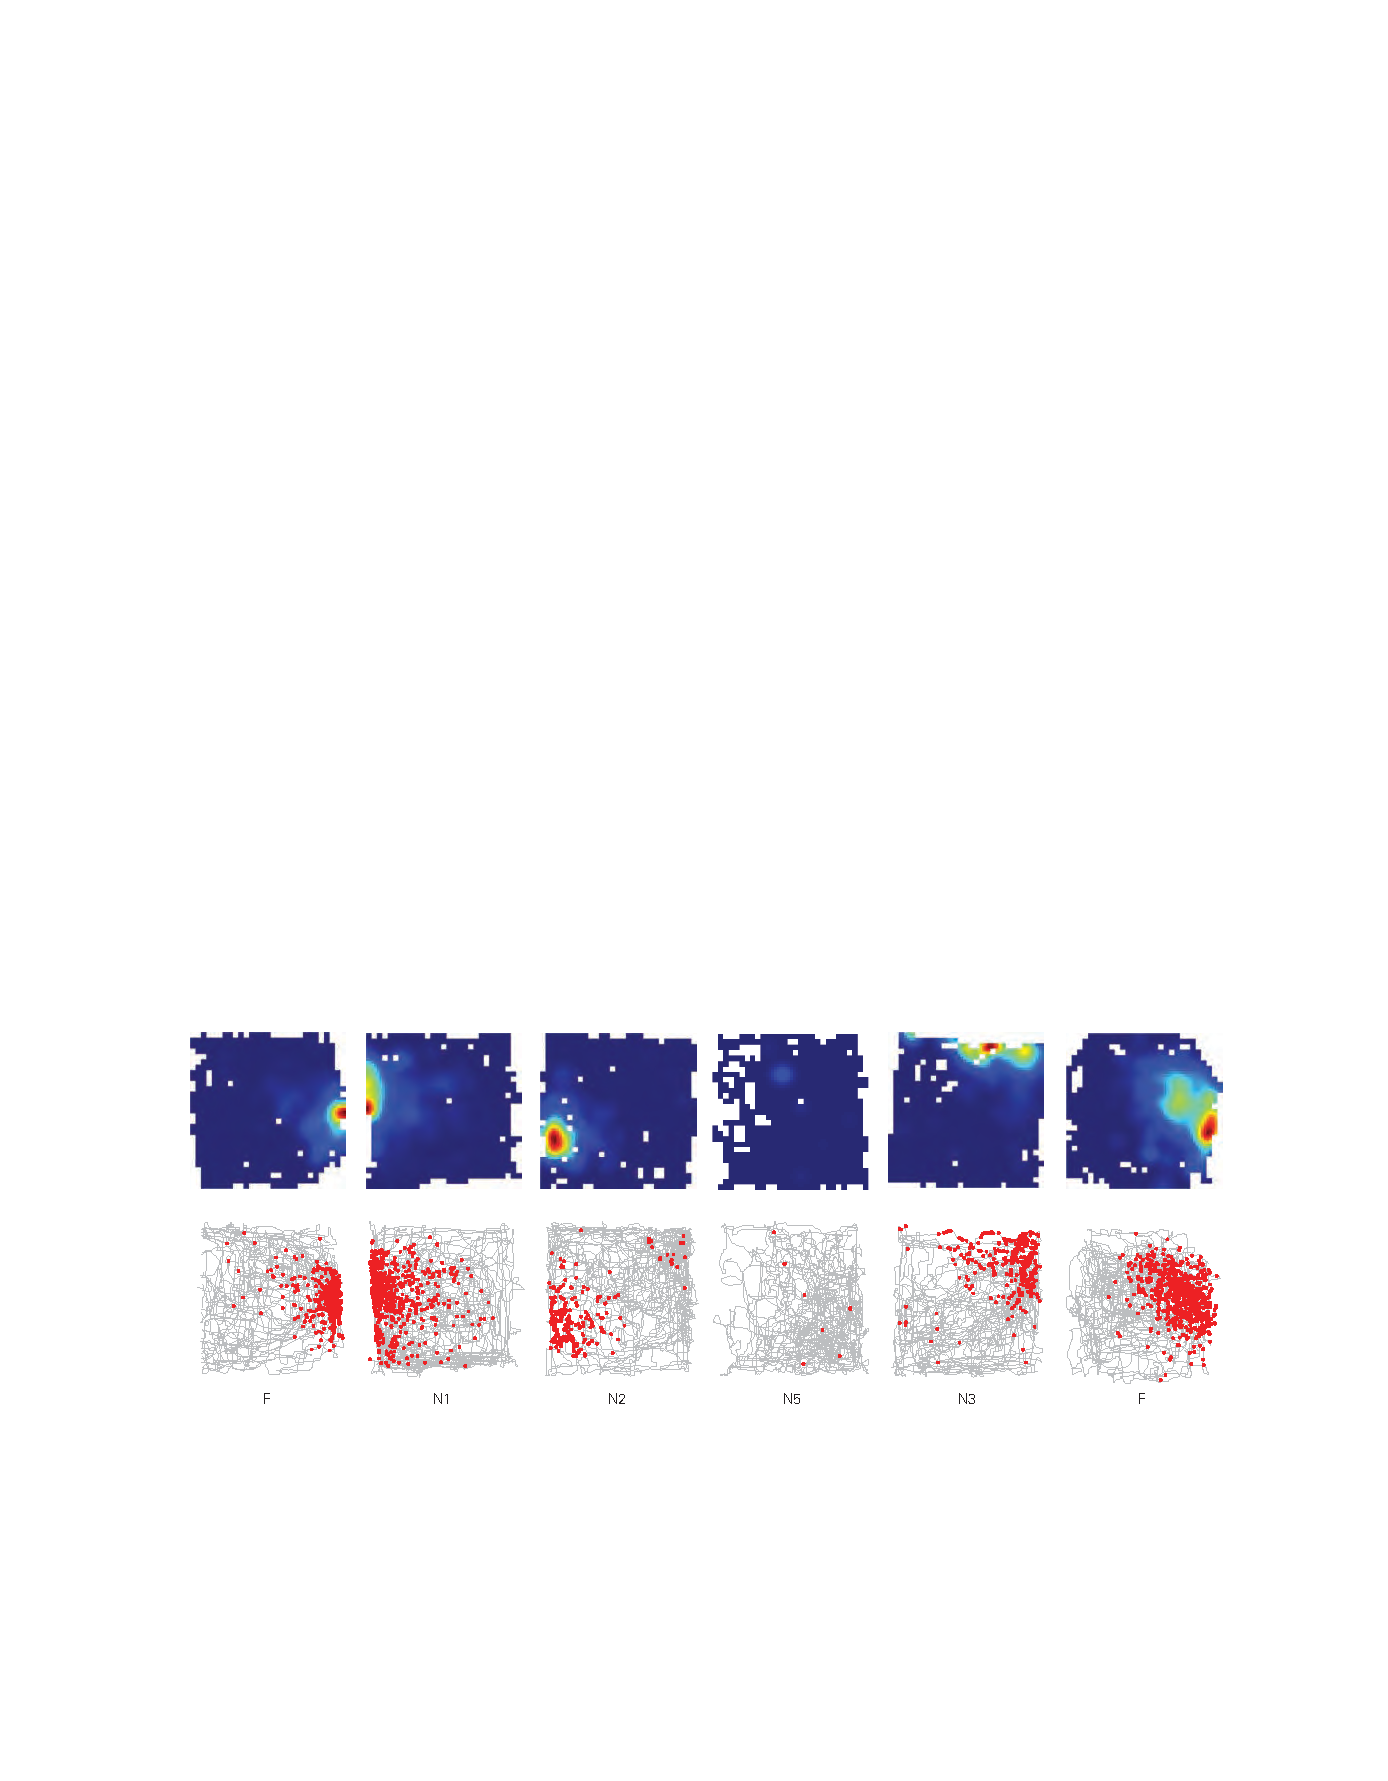
\includegraphics[width=0.9\linewidth]{chap54/fig_54_15}
	\caption{放置单元格为不同的环境形成独立的地图。 速率图显示了不同方形围栏中单个海马体位置细胞的放电模式,每个围栏位于不同的房间。 大鼠在一个熟悉的 (F) 和 11 个新的 (N) 房间中进行了测试(仅显示了四个新房间的录音)。 顶行显示射击率图,而底行显示动物移动的轨迹,射击位置为红色。 该单元仅在某些房间(F、N1、N2、N3)中处于活动状态,这些房间的射击位置不同。 当大鼠在实验结束时返回熟悉的房间时,细胞的发射场与熟悉房间中的初始记录位置相似,表明给定细胞在相同环境中的空间发射模式是稳定的。 (经许可改编自 Alme 等人,2014 年。)}
	\label{fig:54_15}
\end{figure}



\subsection{位置细胞是空间记忆基质的一部分}

除了代表动物的当前位置外,位置细胞还被认为以位置相关的放电模式存储位置记忆,这些模式是在没有最初引发放电的感觉输入的情况下被诱发的。
例如,当动物沿着线性迷宫反复跑几圈后进入睡眠状态时,放置细胞会以与在迷宫中相同的顺序自发放电,这种现象称为“重播”。
同样,过去的轨迹和经验可能会影响环境中特定位置的发射率。
位置细胞代表过去经历的事件和位置的能力可能是海马体编码事件复杂记忆能力的基础。


一旦针对给定环境形成了海马神经元群的放电模式,它是如何维持的?
因为位置细胞是接受实验性 LTP 的相同海马锥体神经元,所以一个自然的问题是 LTP 是否重要。
这个问题在 LTP 被破坏的小鼠实验中得到解决。


在缺乏\textit{N-甲基-D-天冬氨酸}受体的 NR1 亚基的小鼠中,尽管 LTP 被阻断,海马锥体神经元仍然在原位场中放电。
因此,将空间感官信息转换为位置场不需要这种形式的 LTP。
然而,突变小鼠的位置域比正常动物的位置域更大,轮廓更模糊。
在突变小鼠的第二个实验中,晚期 LTP 和长期空间记忆被编码 PKA 蛋白抑制剂的转基因的表达选择性地破坏。 在这些小鼠中,位置场也形成,但单个细胞的放电模式仅稳定一个小时左右(图 \ref{fig:54_16})。
因此,晚期 LTP 是位置场的长期稳定所必需的,但不是它们的形成所必需的。


\begin{figure}[htbp]
	\centering
	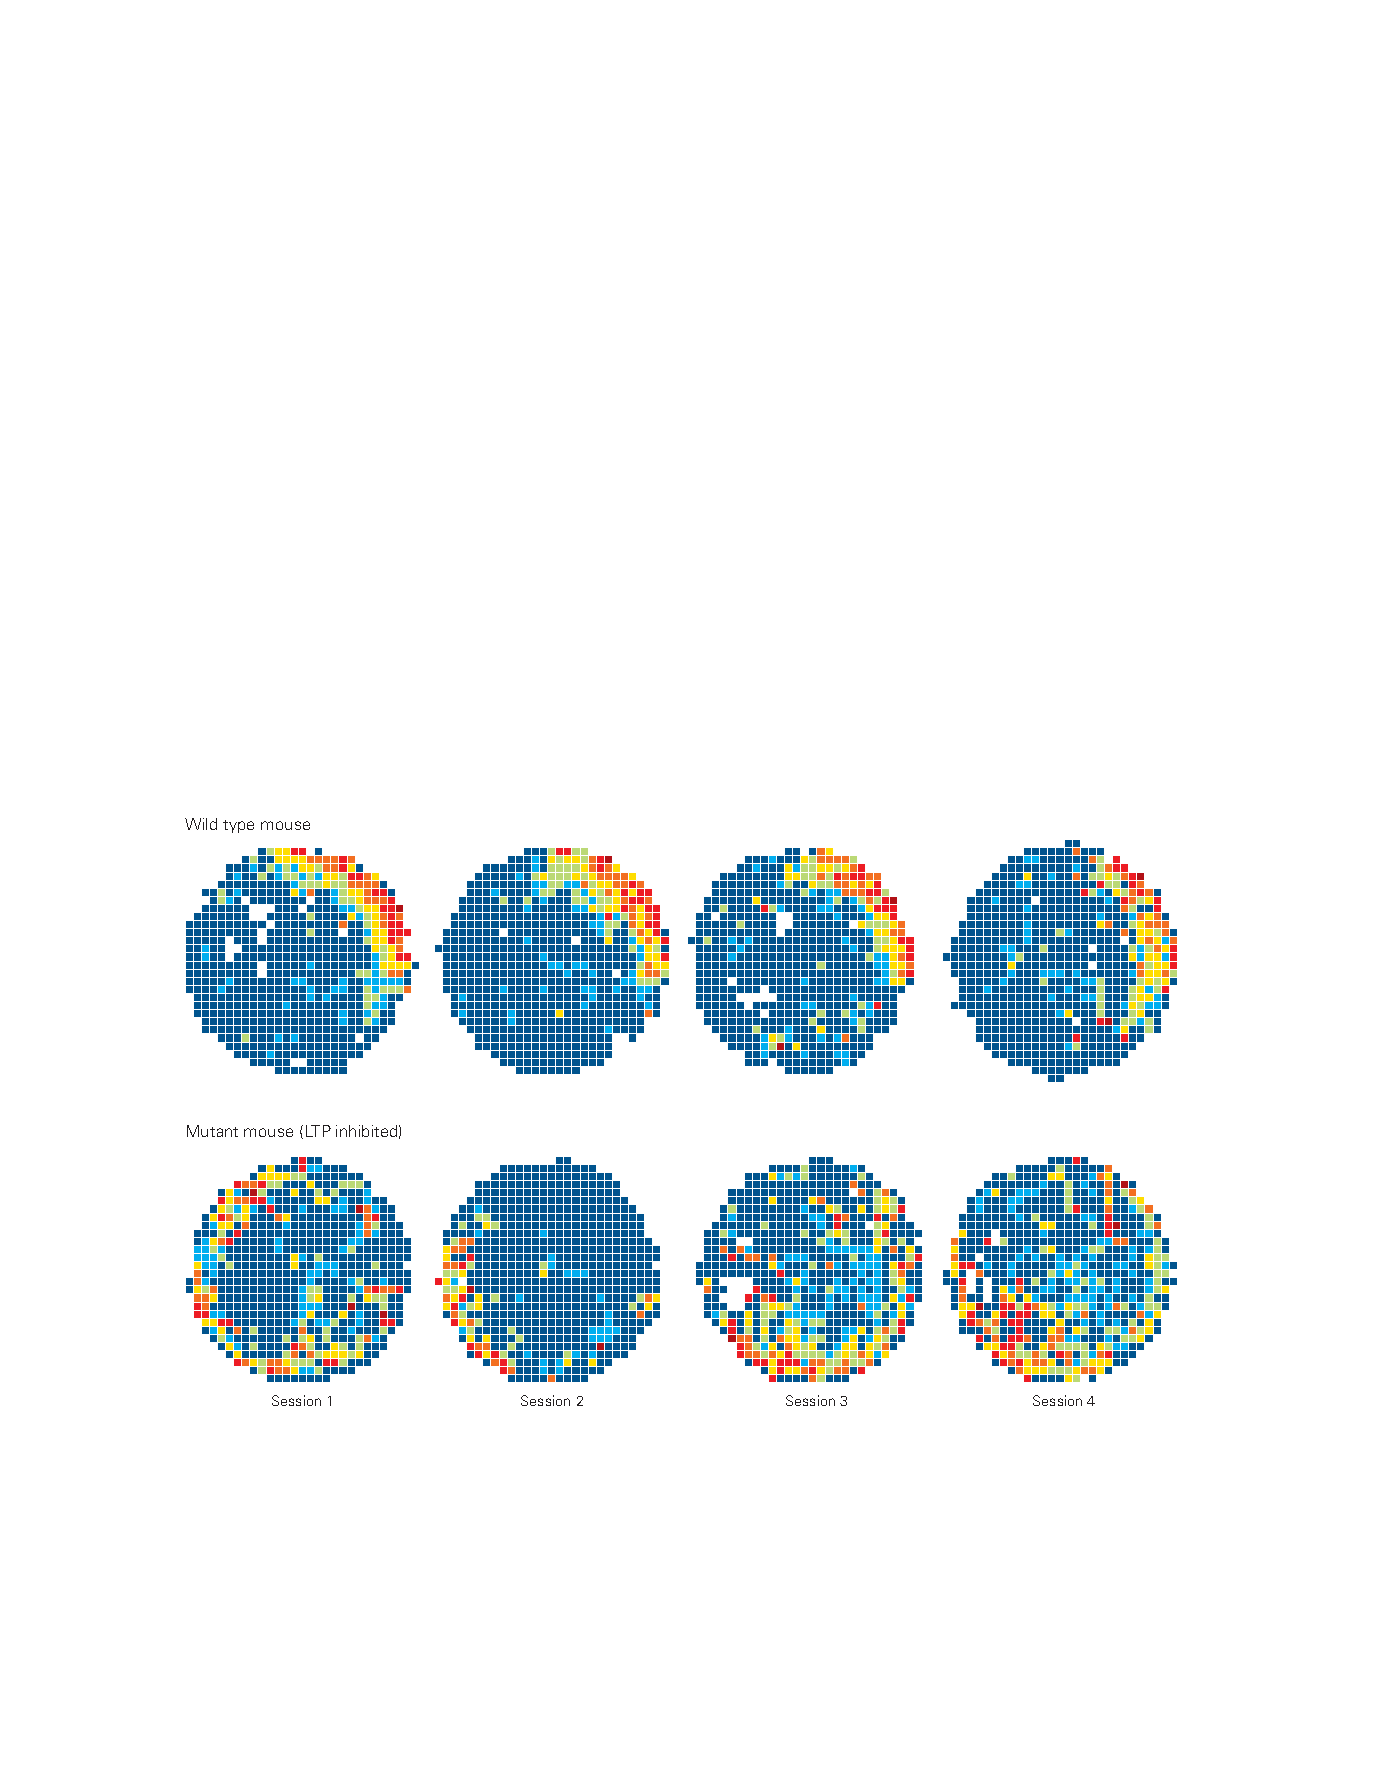
\includegraphics[width=0.9\linewidth]{chap54/fig_54_16}
	\caption{长期增强 (LTP) 的中断会降低海马体中位置场形成的稳定性。 颜色编码的发射率图(参见图 54-12)显示了在野生型小鼠的单个海马锥体神经元和表达持续活跃的 CaMKII(抑制 LTP 的诱导)。 在每次录音之前,动物都会被带出围栏,稍后再重新放回围栏中。 在这四个阶段中的每一个阶段,野生型动物细胞的位置场都是稳定的; 每当动物位于围栏的右上区域时,电池就会启动。 相比之下,突变小鼠细胞的位置域在四个会话中不稳定。 (经许可转载自 Rotenberg 等人,1996 年。)}
	\label{fig:54_16}
\end{figure}


这些动物周围环境的地图在多大程度上调解了外显记忆? 在人类中,外显记忆被定义为有意识地回忆关于人、地点和物体的事实。
虽然意识不能在老鼠身上进行经验研究,但可以检查有意识回忆所需的选择性注意。


当向小鼠呈现不同的行为任务时,位置场的长期稳定性与执行任务所需的注意力程度密切相关。
当鼠标不注意它穿过的空间时,放置场会形成但在 3 到 6 小时后不稳定。
位置场不稳定的动物无法学习空间任务。
然而,当老鼠被迫注意空间时,例如,当训练它跑到特定位置时,位置字段会稳定数天。


这种注意力机制是如何工作的?
对灵长类动物的研究表明前额叶皮层和调节多巴胺能系统在注意力过程中的重要性。
事实上,在小鼠体内形成稳定的位置场需要激活多巴胺 D1/D5 型受体,这已被证明可以通过 cAMP 的产生和 PKA 的激活来增强晚期 LTP 的形成。
这些结果表明,位置场的长期记忆,而不是一种无需有意识地存储和调用的内隐记忆形式,需要动物关注其环境,就像人类的外显记忆一样。



\section{海马体功能紊乱导致的自传体记忆障碍}

我们的认同感在很大程度上取决于我们存储的明确的自传体记忆以及我们在熟悉的空间环境中识别和导航的能力。
破坏这些能力的神经和精神疾病通常是由于海马体和颞叶相关区域的神经回路和可塑性机制发生变化而发生的。


现在有大量证据表明,与阿尔茨海默病相关的毁灭性记忆丧失与蛋白质片段 β-淀粉样蛋白 (Aβ) 的细胞外斑块和微管相关蛋白 tau 的细胞内神经原纤维缠结的积累有关(第 \ref{chap:chap64} 章)。
然而,甚至在斑块和缠结明显之前,可溶性 Aβ 和 tau 水平的升高被认为会破坏许多细胞过程,特别是通过降低某些突触的早期和晚期 LTP 的幅度。
阿尔茨海默病小鼠模型还显示海马体位置细胞稳定性和群体水平同步性发生改变,这可能导致记忆力减退和空间定向障碍。
通过功能磁共振成像研究,在小鼠疾病模型和人类的电生理记录中也观察到了网格细胞功能的变化。
尽管许多临床前研究表明,降低 Aβ 水平的药物可以挽救啮齿动物的突触功能和记忆,但到目前为止,这些治疗方法在治疗阿尔茨海默病患者方面不太成功,这可能是因为必须在早期阶段开始治疗 不可逆的突触变化。


海马体功能改变也可能导致精神分裂症患者出现认知问题,包括工作记忆障碍(第 \ref{chap:chap60} 章)。
最近使用精神分裂症遗传小鼠模型的研究报告称,与工作记忆相关的海马体和前额皮质之间的同步性降低。
此外,海马体 CA1 区位置细胞的位置场在这只小鼠中可能过于僵硬,这表明海马体区分不同环境的能力可能受损。
最后,这些小鼠的社交记忆缺陷与 CA2 区域小白蛋白阳性抑制神经元的减少有关;
在精神分裂症和双相情感障碍患者的死后脑组织中观察到类似的抑制性神经元丢失。


因此,对海马体和相关颞叶结构的研究提供了巨大的希望,可以从根本上深入了解外显记忆是如何存储和回忆的,以及这些结构的功能改变如何导致神经精神疾病。
反过来,这种洞察力可能有助于发现针对这些破坏性疾病的新疗法。



\section{亮点}

1. 外显记忆既有短期成分,称为工作记忆,也有长期成分。
这两种形式都依赖于前额叶皮层和海马体。 


2. 长期记忆被认为依赖于皮质-海马回路中突触的活动依赖性长期突触可塑性。
短暂的强直刺激高频序列导致皮质-海马回路每个阶段的兴奋性突触传递的长时程增强 (LTP)。


3. 许多突触的 LTP 取决于钙流入由\textit{N-甲基-D-天冬氨酸}型谷氨酸受体介导的突触后细胞。
该受体充当巧合检测器:它需要谷氨酸释放和强烈的突触后去极化来传导钙。 


4. LTP 的表达取决于 α-amino-3-hydroxy-5-methyl-4-isoxazolepropionic acid (AMPA) 型谷氨酸受体在突触后膜中的插入或突触前谷氨酸释放的增加,具体取决于 突触的类型和强直刺激的强度。


5. LTP有早期和晚期。 早期 LTP 依赖于共价修饰,而晚期 LTP 依赖于新蛋白质合成、基因转录和新突触连接的生长。


6. 破坏 LTP 的药理学和基因操作通常会导致长期记忆受损,这表明 LTP 可能为记忆存储提供重要的细胞机制。


7. 记忆由细胞集储存。
可能需要 LTP 来形成特定于事件的程序集。
记忆的召回可能反映了在原始事件期间处于活动状态的相同程序集的重新激活。


8. 海马体编码空间和非空间信号。
许多海马神经元充当定位细胞,当动物访问其环境中的特定位置时会发射动作电位。


9. 内嗅皮层是为海马体提供大部分输入的皮层区域,它也对非空间和空间信息进行编码。
内嗅皮层的内侧部分包含称为网格细胞的神经元,当动物穿过六边形网格状空间位置格子的顶点时,这些神经元会激发。
网格单元被组织成具有不同网格频率的半独立半地形组织模块。
内嗅图还包含边界单元、对象矢量单元、头部方向单元和速度单元。


10. 在一个网格单元模块内,成对的网格单元在环境和体验中保持严格的触发关系,这表明网格单元形成了一个在所有环境中都以类似方式表达的通用地图。
相比之下,海马体中的细胞形成塑料地图,因为它们在环境之间完全不相关。


11. 阿尔茨海默病和精神分裂症等神经精神疾病与海马和内嗅突触功能、位置细胞特性以及学习和记忆的缺陷有关。
旨在恢复这种功能的治疗可能会产生新的疾病治疗方法。 


12. 尽管存在明显差异,但隐式(第 \ref{chap:chap53} 章)和显式内存存储依赖于共同的逻辑。
用于存储内隐记忆的活动依赖性突触前促进和用于存储外显记忆的关联长期增强都依赖于特定蛋白质的关联特性:
内隐记忆中的腺苷酸环化酶激活需要神经递质加上细胞内 Ca2+,而外显记忆中的\textit{N-甲基-D-天冬氨酸}受体激活需要谷氨酸 加上突触后去极化。
这种相似性表明联想学习规则对记忆存储的根本重要性。






